\documentclass[11pt,a4paper]{article}

% Paquets de base
\usepackage[utf8]{inputenc}
\usepackage[T1]{fontenc}
\usepackage{lmodern}
\usepackage{microtype}
\usepackage[shorthands=off,french]{babel}
\usepackage[a4paper,margin=2.2cm]{geometry}
\usepackage{amsmath,amssymb,mathtools}
\usepackage{graphicx}
\graphicspath{{../}} % les figures sont dans reports/figures
\usepackage{booktabs}
\usepackage{array}
\usepackage{tabularx}
\usepackage{multirow}
\usepackage{makecell}
\usepackage{enumitem}
\usepackage{xcolor}
\usepackage{float}
\usepackage{caption}
\usepackage{subcaption}

% Pseudocode
\usepackage{algorithm}
\usepackage{algpseudocode}
\algrenewcommand\algorithmicrequire{\textbf{Entrée :}}
\algrenewcommand\algorithmicensure{\textbf{Sortie :}}

% Références et Liens
\usepackage[hyphens]{url}
\usepackage{hyperref}
\usepackage[nameinlink,capitalise]{cleveref}

\hypersetup{
  colorlinks=true,
  linkcolor=blue!55!black,
  citecolor=blue!55!black,
  urlcolor=blue!65!black,
  pdftitle={Au-delà des heuristiques de dispatching statiques},
  pdfauthor={Jean-Luc MUPASA KALUNGA}
}

% Configuration des légendes et tableaux
\captionsetup{font=small,labelfont=bf} % Légendes petites et labels en gras
\setlist[itemize]{leftmargin=1.5em,itemsep=2pt,topsep=4pt}
\setlist[enumerate]{leftmargin=1.7em,itemsep=2pt,topsep=4pt}
\renewcommand{\arraystretch}{1.15} % Espacement vertical des tableaux

% Suppression du style fancyhdr
\pagestyle{plain} 

% Macros de rédaction (optionnelles, mais gardées pour votre travail)
\newcommand{\pending}[1]{\textcolor{red}{[À COMPLÉTER : #1]}}
\newcommand{\tbd}{\textcolor{red}{\textit{À DÉFINIR}}}
% Cadre de figure provisoire (a remplacer par \includegraphics)
\newcommand{\phfig}[2][6cm]{%
  \fbox{\parbox[c][#1][c]{0.92\textwidth}{\centering\textit{#2}}}}

% Titre et Auteurs
\title{\textbf{Au-delà des heuristiques de dispatching statiques : une évaluation comparative de l'apprentissage par renforcement profond face aux perturbations dans l'exploitation minière à ciel ouvert}}

\author{%
\begin{tabular}{c}
Jean-Luc Mupasa Kalunga$^{1}$ \qquad Olfa Ferchichi$^{2}$\\[0.5em]
{\small $^{1}$Faculté d'Informatique, Université Don Bosco de Lubumbashi (UDBL), Lubumbashi, RDC}\\
{\small $^{2}$Laboratoire RIADI, ENSI, Université de la Manouba, Tunis, Tunisie}\\[0.3em]
{\small\texttt{16mk293@esisalama.org; olfaferchichi@yahoo.fr}}
\end{tabular}%
}
\date{} % Pas de date apparente


\begin{document}

\maketitle

\begin{abstract}
Les systèmes camions--pelles représentent jusqu'à 60\,\% des coûts d'exploitation totaux d'une mine à ciel ouvert
et sont extrêmement sensibles aux perturbations opérationnelles. Les heuristiques de dispatching statiques restent la
norme dans l'industrie, et les travaux existants sur l'apprentissage par renforcement évaluent généralement les politiques
dans un seul régime de fonctionnement, ce qui laisse la résilience des agents adaptatifs face aux perturbations mal
caractérisée. Cet article évalue la performance et la robustesse opérationnelle de huit politiques de dispatching :
quatre heuristiques classiques, deux agents d'apprentissage par renforcement tabulaire (Q-Learning, SARSA) et deux agents
d'apprentissage par renforcement profond (Deep Q-Network (DQN), Proximal Policy Optimization (PPO)), dans trois scénarios :
conditions nominales, sursaturation de la flotte et fréquence élevée de pannes d'équipements. Quatre indicateurs de
performance principaux sont évalués (productivité, temps d'attente moyen, taux d'utilisation des équipements et consommation
spécifique de carburant) à partir de 30 réplications indépendantes par couple (politique, scénario) et de tests statistiques
corrigés (analyse de variance de Welch / Kruskal--Wallis, correction de Holm--Bonferroni). Trois résultats principaux
se dégagent. Premièrement, PPO atteint la productivité nominale la plus élevée (4\,176,7~t/h, soit $+2{,}6\,\%$ par rapport à l'Affectation fixe,
$p < 0{,}001$, $d=1{,}94$). Deuxièmement, un effondrement par congestion propre aux heuristiques fondées sur la distance est
identifié en situation de sursaturation de la flotte : Pelle la plus proche et Plus court chemin atteignent des temps d'attente proches de 200 minutes par cycle, tandis que
les agents fondés sur les files d'attente et les agents d'apprentissage par renforcement profond restent en dessous de 100 minutes. Troisièmement, DQN
fournit le débit observé le plus élevé en conditions de pannes fréquentes (3\,949,2~t/h), devançant l'Affectation fixe de 130,7~t/h (Dunn $p=5{,}78\times10^{-3}$, $d=1{,}896$) ; son avantage de 49,6~t/h sur PPO n'est pas significatif avec le test post-hoc fondé sur les rangs ($p=0{,}686$). Ces résultats montrent que les bénéfices de l'apprentissage par renforcement profond pour le dispatching des camions
dépendent fortement du régime de fonctionnement, et ne sont pas systématiquement supérieurs à ceux des heuristiques conventionnelles.
PPO offre la productivité la plus élevée en conditions nominales, tandis que l'Affectation fixe demeure très compétitive
en cas de sursaturation de la flotte, et que DQN présente le débit absolu le plus élevé en cas de pannes fréquentes d'équipements.
L'inversion observée du classement des politiques selon les régimes de fonctionnement met en évidence les limites de l'évaluation
à scénario unique et plaide en faveur d'un recours aux tests de résistance multi-régimes pour évaluer la résilience opérationnelle
des politiques intelligentes de gestion de flotte.
\end{abstract}

\noindent\textbf{Mots-clés :} Apprentissage par renforcement profond ; Exploitation minière à ciel ouvert ; Dispatching de camions ; Gestion de flotte ; Résilience opérationnelle ; Simulation stochastique ; PPO ; DQN.

% ============================================================================
% Section 1: Introduction
% ============================================================================
\section{Introduction}
\label{sec:intro}

L'exploitation minière à ciel ouvert constitue une pierre angulaire de la chaîne mondiale d'approvisionnement en matières premières, où la viabilité économique des opérations est indissociable de l'efficacité de systèmes logistiques de grande envergure. Il est par conséquent impératif d'explorer les avancées technologiques récentes pour améliorer la performance et la résilience de ces dispositifs logistiques.

% ---------------------------------------------------------
\subsection{Contexte industriel}
% ---------------------------------------------------------

Les mines à ciel ouvert sont des systèmes industriels de très grande échelle dans lesquels le cycle camions--pelles constitue l'ossature logistique principale. Ce processus, qui comprend l'excavation, le transport et le déversement des matériaux, n'est pas une simple tâche opérationnelle mais un facteur financier déterminant, représentant jusqu'à 60\,\% des coûts d'exploitation totaux d'un site minier \cite{Afrapoli2017}. Dans l'exploitation minière moderne, la pression pour optimiser ces flux est double : maximiser le débit afin de répondre à la demande mondiale de matières premières, tout en minimisant la consommation d'énergie et les émissions de gaz à effet de serre associées aux flottes de transport diesel.

L'efficacité de ces systèmes est toutefois constamment mise à l'épreuve par une forte variabilité opérationnelle. Dans les environnements miniers réels, les conditions sont loin d'être déterministes. Les pannes d'équipements, les fluctuations de charge utile, les temps de trajet aléatoires causés par la dégradation des pistes et les congestions soudaines du trafic créent ensemble un environnement très instable. La gestion de cette complexité exige une prise de décision en temps réel, capable de concilier la productivité immédiate et la résilience à long terme de la flotte.

Cette étude repose sur trois concepts utilisés tout au long de l'article. L'\textit{apprentissage par renforcement} (\textit{Reinforcement Learning}, RL) désigne une branche de l'intelligence artificielle dans laquelle un agent autonome apprend un comportement optimal par essais et erreurs, au fil de ses interactions avec un environnement dynamique, de façon à maximiser un signal de récompense cumulée. L'\textit{apprentissage par renforcement profond} (\textit{Deep Reinforcement Learning}, DRL) étend le RL en intégrant des réseaux de neurones profonds pour approximer les fonctions de valeur ou les politiques, ce qui permet à l'agent de traiter les espaces d'états de grande dimension et continus typiques des infrastructures minières. Le \textit{dispatching de camions} (\textit{truck dispatching}) désigne le processus opérationnel en temps réel consistant à affecter des unités de transport à des points de chargement et de déversement précis afin d'optimiser la synchronisation de la flotte et la productivité.

% ---------------------------------------------------------
\subsection{Problème de recherche}
\label{sec:problem-statement}
% ---------------------------------------------------------

Le défi central du dispatching est l'affectation dynamique, en temps réel, des camions aux points de chargement et de déversement afin d'optimiser un objectif multidimensionnel combinant débit, temps d'inactivité et consommation d'énergie. Les systèmes de gestion de flotte (\textit{fleet management systems}, FMS) sont déployés dans les mines en exploitation depuis plusieurs décennies \cite{Afrapoli2017, AlexandraNewman2010}, et les règles de décision qui les sous-tendent sont bien documentées \cite{MohanMunirathinam1994, Alarie2002}.

Ces systèmes peinent néanmoins face aux non-linéarités induites par les perturbations soudaines. Lorsqu'une pelle tombe en panne ou qu'une piste de transport se congestionne, une perturbation locale se propage dans l'ensemble du réseau de transport, produisant des goulots d'étranglement sous forme de files d'attente, une sous-utilisation d'équipements à forte intensité capitalistique et une consommation excessive de carburant pendant les périodes de ralenti. Des études à événements discrets portant sur la sursaturation de la flotte rapportent cet effet de propagation et montrent que le temps d'attente en file augmente avec la taille de la flotte dès lors que la capacité de chargement de la fosse est dépassée \cite{Zeng2022, NecmettinCetin2004}.

La question pratique qui en découle n'est pas de savoir si un dispatching adaptatif peut améliorer la productivité en conditions stables, mais si une politique adaptative reste préférable lorsque le régime de fonctionnement s'écarte des conditions pour lesquelles elle a été conçue. Répondre à cette question exige de comparer des politiques adaptatives et des politiques à base de règles dans des régimes contrastés, au sein d'un même environnement et d'un même protocole de mesure.

% ---------------------------------------------------------
\subsection{Lacune de la recherche}
\label{sec:gap}
% ---------------------------------------------------------

L'effet de propagation décrit ci-dessus n'a pas été caractérisé pour plusieurs types de perturbations dans des conditions expérimentales identiques. Les revues de la littérature sur la gestion de flotte fondée sur le RL observent que la plupart des contributions restent au stade de preuve de concept et sont évaluées dans des environnements stables \cite{Hazrathosseini2024}, et les études individuelles confirment ce constat : les agents sont entraînés et testés en conditions nominales, face à un petit nombre de règles de référence, et avec un nombre de réplications rarement indiqué \cite{deCarvalho2023, Zhao2025, Pei2025, FranciscoRosales2025}. Il en résulte qu'un praticien ne dispose d'aucun corpus de preuves indiquant dans quelles conditions de fonctionnement une politique de dispatching apprise doit être déployée, et dans quelles conditions une heuristique statique demeure le choix rationnel. La \cref{sec:relwork} examine cette lacune en détail et la \cref{sec:positioning} expose la manière dont la présente étude y répond.

% ---------------------------------------------------------
\subsection{Questions de recherche et hypothèses}
\label{sec:rq}
% ---------------------------------------------------------

L'évaluation empirique répond aux questions de recherche suivantes :

\begin{description}[leftmargin=1.2cm,labelwidth=1.0cm]

  \item[QR1] Quelle politique de dispatching atteint la productivité la plus élevée dans chaque
  scénario opérationnel, et le classement se maintient-il d'un scénario à l'autre ?

  \item[QR2] Comment le compromis entre productivité et temps d'attente évolue-t-il
  des conditions de fonctionnement nominales aux conditions perturbées ?

  \item[QR3] Les écarts de performance observés sont-ils statistiquement significatifs après
  correction pour comparaisons multiples ?

  \item[QR4] Dans quelle mesure les politiques apprises se dégradent-elles lorsqu'elles sont déployées sur des
  régimes de fonctionnement différents de celui utilisé pendant l'entraînement ?

  \item[QR5] Quelle est la stabilité de la performance de chaque politique d'une graine
  aléatoire indépendante à l'autre ?

  \item[QR6] Comment le choix de la politique de dispatching affecte-t-il la consommation spécifique de
  carburant par tonne transportée, et le classement sur cette dimension suit-il
  le classement de productivité ?

\end{description}

La QR1 est traitée dans la \cref{sec:results}, la QR2 dans la \cref{sec:waiting}, les QR3 et QR4 dans la \cref{sec:robustness} et l'analyse statistique qui la suit, la QR5 dans la \cref{sec:stability} et la QR6 dans la \cref{sec:sustainability}.

Pour guider cette investigation, nous formulons quatre hypothèses réfutables :

\begin{itemize}
  \item \textbf{H1 :} Les politiques d'apprentissage par renforcement profond offrent une productivité supérieure à celle des heuristiques industrielles statiques en conditions de fonctionnement nominales.
  \item \textbf{H2 :} En cas de perturbations opérationnelles, les politiques d'apprentissage par renforcement profond présentent une moindre dégradation du temps d'attente que les heuristiques statiques ; leur avantage sur le débit brut en tonnage dépend du régime et n'est pas garanti dans tous les scénarios.
  \item \textbf{H3 :} La politique de dispatching optimale dépend du régime ; aucun algorithme ne domine dans tous les états opérationnels (nominal, forte charge et fortes pannes).
  \item \textbf{H4 :} Une productivité élevée n'est pas nécessairement corrélée à une faible congestion, ce qui suggère l'existence d'un compromis de Pareto entre le débit et les temps d'attente.
\end{itemize}

% ---------------------------------------------------------
\subsection{Contributions}
\label{sec:contributions}
% ---------------------------------------------------------

Ce travail apporte quatre contributions à l'ingénierie minière et à la gestion intelligente de flotte. Elles sont défendues face à la littérature existante dans la \cref{sec:positioning} et instrumentées dans les sections \cref{sec:design} et \cref{sec:results}.

\begin{itemize}
  \item \textbf{C1. Cadre d'évaluation multi-régimes reproductible.} Un simulateur stochastique compatible Gymnasium est associé à un protocole de mesure standardisé comprenant 30 réplications indépendantes par couple (politique, scénario), des graines aléatoires communes pour la réduction de la variance, des tests omnibus et post-hoc corrigés, et des intervalles de confiance par bootstrap. À notre connaissance, il s'agit de l'un des premiers bancs d'essai librement accessibles pour le dispatching camions--pelles qui couvre à la fois la sursaturation de la flotte et les pannes d'équipements.

  \item \textbf{C2. Banc d'essai comparatif inter-familles de huit politiques.} Quatre heuristiques industrielles statiques (FIFO, Affectation fixe, Pelle la plus proche, Plus court chemin), deux agents d'apprentissage par renforcement tabulaire (Q-Learning, SARSA) et deux agents d'apprentissage par renforcement profond (DQN, PPO) sont évalués dans trois scénarios opérationnels. Les huit politiques observent le même état, agissent sur le même ensemble d'actions et sont évaluées avec les mêmes indicateurs.

  \item \textbf{C3. Identification mécaniste de l'effondrement par congestion.} Une analyse du comportement d'affectation fondée sur l'entropie identifie le mécanisme de point chaud des files d'attente par lequel les heuristiques fondées sur la distance échouent en cas de sursaturation de la flotte, et le distingue des logiques de dispatching fondées sur les files d'attente et des logiques apprises, qui contiennent la congestion.

  \item \textbf{C4. Découplage empirique entre efficacité nominale et résilience opérationnelle.} Le classement des politiques de dispatching s'avère s'inverser d'un régime à l'autre, de sorte que la productivité nominale est un mauvais prédicteur de la robustesse face aux perturbations. Ce résultat a des implications directes pour la conception des protocoles d'évaluation des systèmes de gestion de flotte minière.
\end{itemize}

Le reste de l'article est organisé comme suit. La \cref{sec:relwork} (\nameref{sec:relwork}) passe en revue la littérature sur le dispatching de camions selon trois paradigmes. La \cref{sec:positioning} (\nameref{sec:positioning}) précise le positionnement de l'étude par rapport à cette littérature. La \cref{sec:formulation} (\nameref{sec:formulation}) formalise le problème de dispatching. La \cref{sec:framework} (\nameref{sec:framework}) décrit le cadre proposé, la \cref{sec:design} (\nameref{sec:design}) le plan expérimental, et la \cref{sec:results} (\nameref{sec:results}) les résultats. La \cref{sec:discussion} (\nameref{sec:discussion}) discute les résultats, et la \cref{sec:conclusion} (\nameref{sec:conclusion}) conclut l'article.

\section{Travaux connexes}
\label{sec:relwork}

L'optimisation des systèmes camions--pelles est au c\oe ur de l'ingénierie minière et de la recherche opérationnelle depuis plus de six décennies. Comme le souligne Newman et al. \cite{AlexandraNewman2010}, l'évolution de ces systèmes est passée de la planification manuelle à des systèmes de gestion de flotte (FMS) automatisés complexes. Cette section passe en revue la littérature autour de trois grands paradigmes : les heuristiques statiques, la programmation mathématique et le domaine émergent de l'apprentissage par renforcement.

\subsection{Dispatching de camions statique et à base de règles}

Le dispatching à base de règles demeure le paradigme dominant dans les mines en exploitation, car il est transparent, peu coûteux en calcul et facile à intégrer dans les logiciels FMS commerciaux. Les premières revues des stratégies de dispatching informatisées \cite{MohanMunirathinam1994} et l'aperçu ultérieur des stratégies de résolution proposé par Alarie et Gamache \cite{Alarie2002} identifient un petit ensemble de règles de décision récurrentes qui structurent encore aujourd'hui la pratique industrielle.

Quatre règles sont particulièrement pertinentes pour la présente étude. \textit{First-In-First-Out} (FIFO) affecte chaque camion disponible à l'unité de chargement dont la demande est en attente depuis le plus longtemps, ce qui garantit l'équité mais ignore la configuration spatiale de la fosse. \textit{L'Affectation fixe} attribue chaque camion à une pelle prédéterminée pour toute la durée du poste ; elle stabilise le facteur d'appariement (\textit{match factor}) et reste une référence industrielle très répandue. Elle ne peut pas réallouer dynamiquement la capacité en réponse à des déséquilibres de files d'attente, mais une réaffectation de secours vers l'unité opérationnelle la plus proche est déclenchée automatiquement si la pelle assignée tombe en panne (voir le Tableau~\ref{tab:baselines} pour la définition opérationnelle précise). \textit{La Pelle la plus proche} envoie le camion vers l'unité de chargement disponible la plus proche, minimisant la distance parcourue à vide au prix d'une optimisation purement locale. \textit{Le Plus court chemin} généralise cette idée en sélectionnant la destination qui minimise le temps de trajet estimé sur le graphe des pistes de transport plutôt que la distance euclidienne.

La performance pratique de ces règles a été évaluée aussi bien sur le terrain qu'en simulation. Subtil et al. \cite{Subtil2011} rapportent une mise en œuvre pratique du dispatching dans une mine à ciel ouvert en exploitation, tandis que Mohtasham et Mirzaei-Nasirabad \cite{MehrnazMohtasham2023} évaluent un progiciel de dispatching commercial dans la mine de cuivre de Sungun et soulignent la sensibilité de la logique à base de règles aux conditions opérationnelles. La simulation à événements discrets a été l'instrument standard de ce type d'évaluation \cite{NecmettinCetin2004, MarceloFioroni2008, Zeng2022, MiladAbolghasemian2020}. Elle montre de façon constante que les règles gloutonnes se dégradent fortement dès que la taille de la flotte dépasse la capacité de chargement de la fosse, car les files d'attente se concentrent sur un sous-ensemble de pelles. C'est précisément ce mécanisme de dégradation que le scénario de forte charge de la présente étude est conçu pour mettre en évidence. Notamment, les quatre règles retenues ici comme références représentent deux logiques de dispatching fondamentalement différentes : les règles fondées sur les files d'attente (FIFO, Affectation fixe) ignorent la géométrie de la fosse mais gèrent l'ordre de service, tandis que les règles fondées sur la distance (Pelle la plus proche, Plus court chemin) s'appuient sur la proximité spatiale sans tenir compte de l'état des files d'attente. Ce contraste est essentiel pour isoler la logique de dispatching responsable des différences de résilience face aux perturbations.

\subsection{Optimisation mathématique et métaheuristiques}

Pour dépasser les limites des règles simples, les chercheurs se sont tournés vers la programmation mathématique. Soumis et al. \cite{Soumis1989} ont proposé une approche à plusieurs étapes combinant la programmation linéaire (PL) pour la planification de la production et des modèles d'affectation pour le dispatching en temps réel. Cette structure modulaire reste l'ossature de nombreux FMS modernes. Ahangaran et al. \cite{Ahangaran2012} ont étendu cette approche en développant des modèles spécifiquement dédiés aux flottes de camions de capacités hétérogènes, en utilisant des réseaux de flots pour équilibrer la production.

Cependant, la nature déterministe de la programmation linéaire en nombres entiers mixtes (MILP) entre souvent en conflit avec la réalité stochastique de l'exploitation minière. Ta et al. \cite{ChungTa2013} ont tenté de combler cet écart en incorporant des probabilités d'inactivité des pelles dans des modèles linéaires, en recourant à la théorie des files d'attente pour obtenir de meilleures estimations de production. Malgré ces avancées, les modèles MILP souffrent fréquemment de la malédiction de la dimensionnalité lorsqu'ils sont appliqués à de grandes mines exploitant des dizaines de camions \cite{AmandaSmith2020, ZhongxinWang2022}.

Pour gérer cette complexité, les métaheuristiques ont été largement appliquées au dispatching et à l'acheminement des camions. Souza et al. \cite{Souza2010} ont démontré qu'une heuristique hybride combinant GRASP et VNS pouvait obtenir des solutions quasi optimales en des temps de calcul réduits. Liu et Chai \cite{GuangweiLiu2019} ont utilisé un algorithme génétique pour minimiser la consommation d'énergie liée au transport tout en tenant compte de la résistance variable des pistes dans le temps. Les algorithmes d'optimisation par colonies de fourmis, qui modélisent la sélection probabiliste d'itinéraires par les insectes sociaux au moyen de mécanismes de mise à jour des phéromones, ont été appliqués aux problèmes d'affectation multi-véhicules dans l'exploitation minière de surface, car leur sélection stochastique s'adapte naturellement aux demandes concurrentes sur des tronçons de piste partagés \cite{ShivPrakashUpadhyay2017}. Le recuit simulé, qui accepte des mouvements sous-optimaux avec une probabilité contrôlée par une température afin d'échapper aux optima locaux, a de même été utilisé pour l'ordonnancement dans les environnements à ciel ouvert \cite{BurakOzdemir2019}. Bien que puissantes, les métaheuristiques sont souvent formulées pour optimiser un état donné du système ou un horizon de planification donné. Lorsque des perturbations importantes modifient les conditions de fonctionnement sous-jacentes, le processus d'optimisation doit être répété ou réoptimisé, ce qui peut limiter la réactivité lorsque les décisions doivent être mises à jour à de courtes échelles de temps dans des environnements miniers dynamiques.

\subsection{Approches par apprentissage par renforcement}

Le passage à l'apprentissage par renforcement représente un changement de paradigme : au lieu de résoudre un nouveau problème d'optimisation à chaque époque de décision, un agent apprend une politique qui associe les états du système à des actions optimales \cite{RichardSutton2018, MoezKrichen2022}. Les premières applications du RL en logistique, comme celles de Nazari et al. \cite{MohammadrezaNazari2018} pour le problème de tournées de véhicules (VRP) et de Zhang et al. \cite{CongZhang2020} pour l'ordonnancement d'atelier (\textit{job-shop}), ont démontré que le DRL pouvait surpasser les heuristiques classiques en apprenant à partir de milliers d'interactions simulées.

Au sein de la famille de l'apprentissage par renforcement, les méthodes diffèrent substantiellement par leur puissance de représentation et leur paradigme d'apprentissage. Les méthodes tabulaires (Q-Learning et SARSA \cite{RichardSutton2018}) construisent des fonctions de valeur sur des tables d'états-actions discrets, ce qui les rend transparentes et légères en calcul, mais leur expressivité se dégrade fortement lorsque l'espace d'observation croît avec la taille de la flotte. Les Deep Q-Networks (DQN) répondent à ce problème en approximant la fonction Q par un réseau de neurones et en stabilisant l'entraînement grâce au rejeu d'expériences et au gel du réseau cible, ce qui permet de généraliser à des entrées continues de grande dimension. La Proximal Policy Optimization (PPO) \cite{JohnSchulman2017} appartient à la famille acteur-critique : elle optimise directement la politique via un objectif de substitution dont la contrainte d'écrêtage (\textit{clipping}) empêche les mises à jour catastrophiques des paramètres. Ces quatre algorithmes, allant du tabulaire au profond, et de l'approche fondée sur la valeur au gradient de politique, forment un spectre comparatif naturel et constituent précisément la composante RL du banc d'essai conçu dans cette étude.

Dans le secteur minier, cette transition est plus récente. Hazrathosseini et Afrapoli \cite{Hazrathosseini2024} proposent une revue critique, soulignant que, bien que le RL présente un potentiel considérable pour les FMS intelligents, la plupart des études restent au stade de la preuve de concept. de Carvalho et Dimitrakopoulos \cite{deCarvalho2023} ont appliqué un cadre acteur--critique à la planification de la production, montrant que le RL peut traiter efficacement la dynamique de la flotte tout en mettant à jour les objectifs de production.

Des bancs d'essai récents, tels que Mining-Gym \cite{Banerjee2025}, ont commencé à fournir des environnements standardisés pour tester ces algorithmes. Zhao et al. \cite{Zhao2025} ont proposé une approche hiérarchique d'apprentissage par renforcement multi-agent (MARL) pour un dispatching durable, avec un accent sur l'efficacité énergétique, tandis que Pei et al. \cite{Pei2025} et Rosales et Diaz \cite{FranciscoRosales2025} ont exploré le dispatching par apprentissage et le dispatching interprétable pour le transport minier autonome. L'usage d'une aide à la décision fondée sur le RL pour l'ordonnancement industriel hiérarchique dépasse le secteur minier : Szatmari et al.~\cite{KingaSzatmari2025} démontrent des architectures multi-niveaux similaires dans la conduite de procédés chimiques, ce qui suggère que les schémas de conception émergeant dans la recherche sur le dispatching minier ont une large pertinence inter-domaines. Une limite commune à ces études est toutefois leur focalisation sur les conditions nominales. La plupart des agents RL sont entraînés et testés dans des environnements stables ; peu d'études évaluent explicitement le comportement d'un agent DQN ou PPO face à des pannes d'équipements fréquentes ou à des pics de congestion inattendus.

\subsection{Synthèse critique et lacune de la recherche}
\label{sec:synthesis}

La littérature examinée révèle quatre lacunes complémentaires qui motivent la présente étude.

Premièrement, les trois paradigmes passés en revue ci-dessus sont rarement comparés entre eux. Les travaux à base de règles comparent les règles de dispatching entre elles \cite{Alarie2002, MehrnazMohtasham2023, Zeng2022}, la programmation mathématique compare un optimiseur à une règle ou à une formulation en nombres entiers mixtes \cite{Soumis1989, AmandaSmith2020}, et les travaux fondés sur l'apprentissage comparent un agent à un petit nombre de règles de référence \cite{deCarvalho2023, Zhao2025}. La comparaison inter-familles est donc rare, et lorsqu'elle existe, les algorithmes sont évalués sur des environnements, des définitions de récompense ou des configurations de flotte différents, ce qui empêche d'attribuer une différence observée à la logique de dispatching elle-même.

Deuxièmement, le régime de fonctionnement est généralement traité comme un contexte fixe plutôt que comme un facteur expérimental. Les agents d'apprentissage par renforcement dans le secteur minier sont entraînés et testés en conditions nominales \cite{deCarvalho2023, Hazrathosseini2024, Zhao2025}, et les études qui prennent en compte les perturbations ne considèrent qu'un seul type de perturbation, le plus souvent la congestion \cite{Zeng2022}. Un classement rapporté est donc conditionnel à un seul point de fonctionnement, et sa stabilité en dehors de ce point reste inconnue.

Troisièmement, la solidité des références est souvent insuffisante pour étayer les gains rapportés. Les études fondées sur l'apprentissage rapportent des améliorations par rapport à deux ou trois règles de référence \cite{Zhao2025}, et parfois par rapport à aucune \cite{deCarvalho2023}. Lorsque la règle de comparaison est faible, une amélioration n'établit que peu de choses sur la valeur pratique de la politique apprise.

Quatrièmement, le protocole inférentiel est rarement documenté. Le nombre de réplications, le contrôle des graines aléatoires et les corrections pour comparaisons multiples sont rarement rapportés dans la littérature sur le dispatching minier \cite{MehrnazMohtasham2023, MiladAbolghasemian2020, BurakOzdemir2019}, alors que la littérature sur l'apprentissage dans des domaines voisins les rapporte \cite{MohammadrezaNazari2018, CongZhang2020}. Compte tenu de la stochasticité d'un environnement minier, avec des charges utiles variables, des temps de trajet aléatoires et des processus de panne aléatoires, une différence de quelques pour cent observée sur une poignée d'exécutions ne peut être distinguée du bruit d'échantillonnage.

Ces quatre lacunes sont traitées conjointement plutôt que séparément. La présente étude évalue un espace de politiques unique de huit dispatchers au sein d'un même environnement de simulation, traite le régime de fonctionnement comme un facteur expérimental, conserve les heuristiques industrielles comme références compétitives, et applique un protocole de réplication conçu pour l'inférence. La \cref{sec:positioning} développe ce positionnement selon les quatre mêmes axes, et le \cref{tab:litterature} le résume.


% ============================================================================
% TABLEAU DE POSITIONNEMENT
% Contient l'ensemble des travaux cites dans la section 2, groupes par
% famille d'approche (mise en forme reprise du tableau de Mme Ferchichi).
% A placer a la fin de la section 2.4 ou au debut de la section 3.
% ============================================================================

\begin{table}[H]
\centering

\caption{Positionnement de l'étude proposée par rapport à des approches représentatives de dispatching de camions.}
\label{tab:litterature}

\renewcommand{\arraystretch}{1.35}
\setlength{\tabcolsep}{3.2pt}
\footnotesize

\begin{tabularx}{\textwidth}{
>{\raggedright\arraybackslash}p{3.0cm}
>{\centering\arraybackslash}p{1.9cm}
>{\centering\arraybackslash}p{2.2cm}
>{\centering\arraybackslash}p{1.7cm}
>{\centering\arraybackslash}p{1.6cm}
>{\centering\arraybackslash}p{2.0cm}
>{\raggedright\arraybackslash}X
}

\toprule

\textbf{Approche} &
\makecell{\textbf{Optimisation}\\\textbf{formelle}} &
\textbf{Apprentissage} &
\makecell{\textbf{Tests de}\\\textbf{perturbation}} &
\textbf{Références} &
\makecell{\textbf{Protocole de}\\\textbf{réplication}} &
\textbf{Objet de l'évaluation} \\

\midrule

Revues sur le dispatching et la gestion de flotte
\cite{AlexandraNewman2010,MohanMunirathinam1994,Alarie2002,Hazrathosseini2024,Afrapoli2017}
&
s.o.
&
s.o.
&
Non
&
s.o.
&
s.o.
&
Panorama des modèles et algorithmes
\\

\addlinespace

Dispatching à base de règles, terrain et simulation
\cite{Subtil2011,MehrnazMohtasham2023,NecmettinCetin2004,MarceloFioroni2008,MiladAbolghasemian2020}
&
Non
&
Non
&
Non
&
Pratique actuelle
&
Limité
&
Validation sur le terrain ou par événements discrets
\\

\addlinespace

Comparaison de règles selon la taille de la flotte
\cite{Zeng2022}
&
Algorithme génétique
&
Non
&
Congestion
&
4 à 6 règles
&
Limité
&
Comparaison de stratégies d'allocation
\\

\addlinespace

Programmation mathématique
\cite{Soumis1989,Ahangaran2012,ChungTa2013,AmandaSmith2020,ZhongxinWang2022}
&
Oui (PL / MILP)
&
Non
&
Non
&
0 à 2
&
Limité
&
Optimalité en conditions stables
\\

\addlinespace

Métaheuristiques et simulation-optimisation
\cite{Souza2010,GuangweiLiu2019,ShivPrakashUpadhyay2017,BurakOzdemir2019}
&
Oui (recherche heuristique)
&
Non
&
Fondé sur des scénarios
&
MILP ou 1 à 2 règles
&
Limité
&
Solutions de planification quasi optimales
\\

\addlinespace

Dispatching par apprentissage, autres domaines
\cite{MohammadrezaNazari2018,CongZhang2020,KingaSzatmari2025}
&
Non
&
RL profond et hiérarchique
&
Non
&
Heuristiques classiques
&
Oui
&
Performance en tournées et ordonnancement
\\

\addlinespace

Apprentissage par renforcement dans le secteur minier
\cite{deCarvalho2023,Banerjee2025,Zhao2025,Pei2025,FranciscoRosales2025}
&
Non
&
Acteur--critique, MARL, RL interprétable
&
Non
&
0 à 3
&
Limité
&
Dispatching de type preuve de concept
\\

\addlinespace

\textbf{Étude proposée}
&
\textbf{Heuristiques statiques comme références compétitives}
&
\textbf{RL tabulaire et profond (Q-Learning, SARSA, DQN, PPO)}
&
\textbf{Congestion et pannes}
&
\textbf{8 politiques}
&
\textbf{30 réplications, graines communes}
&
\textbf{Résilience opérationnelle multi-régimes}
\\

\bottomrule

\end{tabularx}
% \smallskip\noindent\footnotesize
% Methodological and tooling references (Sutton and Barto \cite{RichardSutton2018}, Krichen \cite{MoezKrichen2022}, Schulman et al.\ \cite{JohnSchulman2017}, Towers et al.\ \cite{MarkTowers2025}, Raffin et al.\ \cite{AntoninRaffin2021}) are omitted from the comparison, since they define algorithms or software rather than comparable dispatching studies.
\end{table}
\section{Positionnement de l'étude}
\label{sec:positioning}

La littérature passée en revue dans la \cref{sec:relwork} aborde le dispatching de camions sous trois angles largement distincts, et le présent travail se situe à leur intersection. Cette section explicite ce positionnement selon les quatre axes introduits dans la \cref{sec:synthesis}, à savoir l'étendue de l'espace de politiques comparé, le traitement des perturbations opérationnelles, la solidité des références et la rigueur inférentielle, avant de préciser ce que l'étude revendique et ce qu'elle ne revendique pas. Le \cref{tab:litterature} présente la même comparaison sous forme de tableau.

% ---------------------------------------------------------
\subsection{Étendue de l'espace de politiques comparé}
% ---------------------------------------------------------

Les études existantes restent généralement à l'intérieur d'une seule famille méthodologique. Les travaux à base de règles \cite{Alarie2002, Subtil2011, MehrnazMohtasham2023, NecmettinCetin2004} comparent des règles de dispatching entre elles ; les travaux sur les métaheuristiques \cite{Souza2010, GuangweiLiu2019, ShivPrakashUpadhyay2017, BurakOzdemir2019} comparent un optimiseur à une règle ou à une formulation en nombres entiers mixtes ; et les travaux fondés sur l'apprentissage \cite{deCarvalho2023, Zhao2025, Pei2025, FranciscoRosales2025} comparent un agent à un petit nombre de règles de référence. Les comparaisons inter-familles sont donc rares, et lorsqu'elles existent, les algorithmes sont généralement évalués sur des environnements, des définitions de récompense ou des configurations de flotte différents, ce qui empêche d'attribuer les écarts de performance à la logique de dispatching elle-même.

Cette étude évalue au contraire un espace de politiques unique de huit dispatchers au sein d'un même environnement de simulation identique. Les quatre heuristiques couvrent les deux logiques industrielles dominantes, fondée sur les files d'attente (FIFO, Affectation fixe) et fondée sur la distance (Pelle la plus proche, Plus court chemin), tandis que les quatre agents d'apprentissage couvrent les dimensions tabulaire et profonde ainsi que les dimensions fondée sur la valeur et gradient de politique de la famille de l'apprentissage par renforcement (Q-Learning, SARSA, DQN, PPO). Comme les huit politiques observent le même état, agissent sur le même ensemble d'actions et sont évaluées avec la même récompense et les mêmes indicateurs clés de performance, la comparaison isole l'effet de la règle de décision plutôt que celui des hypothèses de modélisation.

% ---------------------------------------------------------
\subsection{Traitement des perturbations opérationnelles}
% ---------------------------------------------------------

Le deuxième axe est le régime de fonctionnement dans lequel les politiques sont évaluées. La plupart des études d'apprentissage par renforcement dans le secteur minier entraînent et testent les agents en conditions nominales \cite{deCarvalho2023, Hazrathosseini2024, Zhao2025}, et les études prenant en compte les perturbations qui existent tendent à ne considérer qu'un seul type de perturbation, le plus souvent la congestion \cite{Zeng2022}. En conséquence, le classement rapporté d'une politique est conditionnel à un seul point de fonctionnement, et sa stabilité en dehors de ce point reste inconnue.

La présente étude traite le régime de fonctionnement comme un facteur expérimental plutôt que comme un contexte fixe. Les mêmes politiques entraînées sont évaluées en conditions nominales, en sursaturation de la flotte et en fréquence élevée de pannes d'équipements, sans réentraînement entre les régimes. Cette conception a deux conséquences. Elle met en évidence le mécanisme de propagation par lequel une perturbation locale, telle qu'une pelle en panne ou un tronçon de piste saturé, devient un goulot d'étranglement à l'échelle du système. Elle fait aussi de la robustesse une grandeur mesurable, à savoir la dégradation de chaque indicateur par rapport à la référence nominale. L'évaluation des agents sur des régimes non vus pendant l'entraînement fournit en outre un test direct de transfert \textit{zero-shot} (sans réentraînement), qui est la question pertinente en pratique pour un site minier, où la distribution de déploiement n'est jamais la distribution d'entraînement.

% ---------------------------------------------------------
\subsection{Solidité des références et rigueur inférentielle}
% ---------------------------------------------------------

Une troisième limite récurrente est la solidité de la comparaison. Les études fondées sur l'apprentissage rapportent fréquemment des gains par rapport à deux ou trois règles de référence \cite{Zhao2025}, parfois par rapport à aucune \cite{deCarvalho2023}, et généralement sur un nombre limité d'exécutions de simulation sans correction pour comparaisons multiples. Sous forte stochasticité, avec des charges utiles variables, des temps de trajet aléatoires et des processus de panne aléatoires, une différence de quelques pour cent observée sur une poignée d'exécutions ne peut être distinguée du bruit d'échantillonnage.

Cette étude utilise l'Affectation fixe et les trois autres heuristiques comme références industrielles compétitives plutôt que comme références faibles, et elle applique un protocole de réplication conçu pour l'inférence : 30 réplications indépendantes par couple (politique, scénario), analyse de variance de Welch et tests de Kruskal--Wallis selon les hypothèses distributionnelles, correction de Holm--Bonferroni sur la famille de comparaisons qui en résulte, et tailles d'effet rapportées en complément des valeurs $p$. La variabilité inter-réplications est elle-même traitée comme un résultat, puisqu'une politique dont la performance fluctue d'une graine à l'autre est opérationnellement moins attrayante qu'une politique légèrement moins productive mais plus prévisible.

% ---------------------------------------------------------
\subsection{Revendications et limites de portée}
% ---------------------------------------------------------

La contribution de cet article est évaluative plutôt qu'algorithmique, en ce sens qu'aucun nouvel algorithme d'apprentissage par renforcement n'est proposé. La contribution réside dans une caractérisation contrôlée, multi-régimes et statistiquement corrigée des situations où les politiques de dispatching apprises justifient leur complexité supplémentaire, et dans l'identification des mécanismes, en particulier l'effondrement par congestion propre aux règles fondées sur la distance, qui sont à l'origine des inversions observées dans le classement des politiques.

Trois limites de portée découlent de ce positionnement et sont discutées plus en détail dans la \cref{sec:limitations}. L'évaluation est menée en simulation, de sorte que les ordres de grandeur rapportés sont conditionnels à la configuration de mine modélisée et doivent être lus comme des comparaisons relatives plutôt que comme des prédictions à l'échelle d'un site. Les agents sont des contrôleurs mono-agent, de sorte que les formulations multi-agents coopératives \cite{Zhao2025} sortent de l'espace comparé. Enfin, les trois scénarios représentent des perturbations stylisées ; ils sont conçus pour être interprétables et reproductibles, et non pour reproduire toute la diversité des incidents rencontrés dans une fosse en exploitation.
\section{Formulation du problème}
\label{sec:formulation}

L'objectif de ce travail est de déterminer dans quels régimes opérationnels une politique de dispatching apprise est préférable à une règle industrielle statique, et d'identifier les mécanismes qui sous-tendent les transitions de performance observées.

Le problème est organisé en deux niveaux complémentaires : la décision d'affectation en temps réel à laquelle le dispatcher est confronté à chaque époque de décision, et l'évaluation comparative de règles de décision alternatives dans des régimes de fonctionnement contrastés. Ces deux niveaux ne doivent pas être confondus. Une politique performante au premier niveau en conditions nominales ne l'est pas pour autant en situation de perturbation, ce que le second niveau est précisément conçu pour mettre en évidence.

\begin{quote}
\textbf{Problème P1 -- Décision de dispatching en temps réel.}
Étant donné l'état courant de la mine, comprenant les profondeurs des files d'attente, les positions des camions, la disponibilité des équipements et l'état des pistes, affecter un camion disponible à un couple pelle--point de déversement de manière à maximiser le débit cumulé sur un poste tout en contenant la formation de files d'attente, la famine des pelles et la consommation de carburant.
\end{quote}

\begin{quote}
\textbf{Problème P2 -- Sélection de politique dépendante du régime.}
Étant donné un ensemble de politiques de dispatching candidates et un ensemble de régimes opérationnels, déterminer quelle politique est la plus performante dans chaque régime, et si le classement obtenu en conditions nominales se transpose aux conditions perturbées.
\end{quote}

Le problème P1 est formalisé ci-dessous sous la forme d'un processus de décision markovien, ainsi que l'environnement stochastique dans lequel il s'inscrit. Le problème P2 est traité par le protocole expérimental de la \cref{sec:design} et par les indicateurs de robustesse définis dans la \cref{sec:metrics}.

Le reste de cette section définit le système camions--pelles, le réseau routier stochastique, le processus de décision markovien et la fonction de récompense multi-objectif.

\subsection{Système camions--pelles}

La mine est modélisée comme un système de transport en boucle fermée composé de trois entités physiques principales :

\begin{enumerate}
  \item \textbf{Unités de chargement (pelles) :} ressources fixes ou semi-mobiles caractérisées par leur cadence et leur capacité de chargement. Chaque pelle est associée à une file d'attente dans laquelle les camions patientent lorsque la ressource est occupée.
  \item \textbf{Unités de transport (camions) :} une flotte homogène ou hétérogène chargée du transport des matériaux. Les camions sont définis par leur capacité, leurs profils de vitesse (à vide ou chargés) et leurs taux de consommation de carburant.
  \item \textbf{Unités de déversement (verses/concasseurs) :} les destinations finales des matériaux. Comme les pelles, ces sites peuvent se congestionner et ont des cadences de service spécifiques.
\end{enumerate}

Le système est soumis à des perturbations opérationnelles, en particulier des pannes d'équipements. Un événement de panne suit une distribution stochastique (par exemple de Poisson ou de Bernoulli), qui retire temporairement un camion ou une pelle de la flotte active et oblige le système de dispatching à réallouer les ressources restantes afin de maintenir les objectifs de production.

\subsection{Réseau routier stochastique}

L'infrastructure de la mine est représentée par un graphe orienté $G = (V, E)$, où :

\begin{itemize}
  \item $V$ (nœuds) représente les points de chargement, les sites de déversement, les intersections et les aires de stationnement ;
  \item $E$ (arêtes) représente les pistes de transport reliant ces points.
\end{itemize}

Contrairement aux modèles déterministes, nous définissons le temps de trajet $T(e)$ de toute arête $e$ comme une variable aléatoire suivant une loi log-normale :

\begin{equation}
T(e) \sim \mathrm{Lognormal}\big(\mu_e, \sigma_e^2\big), \qquad e \in E .
\end{equation}

Cela rend compte de la variabilité intrinsèque des temps de trajet causée par l'état des pistes, le comportement des conducteurs et les interactions entre véhicules. En outre, le modèle intègre la dégradation des pistes, selon laquelle l'état d'un tronçon peut se détériorer au fil du temps, affectant les vitesses moyennes de déplacement jusqu'à ce qu'une maintenance soit effectuée.

\subsection{Processus de décision markovien}

Le problème de dispatching de camions est formulé comme un processus de décision markovien (MDP) défini par le n-uplet $(S, A, P, R, \gamma)$. La \cref{fig:mdp} illustre la boucle d'interaction agent--environnement ; le \cref{tab:mdp} résume les définitions des composantes.

\subsubsection{Espace d'états}

L'état $S_t$ à l'instant $t$ fournit un instantané complet de la mine. Il est représenté par un vecteur de grande dimension dont la taille suit la formule $15 + 11 \times N$, où $N$ est la taille de la flotte (147 dimensions pour les scénarios nominal et de fortes pannes avec $N=12$ ; 213 dimensions pour le scénario de forte charge avec $N=18$). Il comprend :

\begin{itemize}
  \item \textbf{État de la flotte :} positions, tâches en cours (transport, retour, attente en file) et charges utiles restantes de tous les camions.
  \item \textbf{Disponibilité des équipements :} état opérationnel des pelles et des sites de déversement (actif ou en panne).
  \item \textbf{Dynamique des files d'attente :} longueur courante et temps d'attente estimés à tous les points de chargement et de déversement.
  \item \textbf{Contexte temporel :} le temps de simulation courant et l'état du réseau routier.
  \item \textbf{Événements opérationnels :} indicateurs de perturbations ou de pannes d'équipements récentes.
\end{itemize}

\subsubsection{Espace d'actions}

L'action $A_t$ est déclenchée chaque fois qu'un camion devient « disponible pour affectation » (typiquement après avoir terminé un cycle de déversement ou au début d'un poste). Chaque action code une \emph{affectation de trajet complète} : un couple pelle--déversement précis $(\text{Pelle}_j, \text{Verse}_k)$ vers lequel le camion est acheminé, ou une attente explicite (WAIT). Avec $S=3$ pelles et $D=2$ sites de déversement, l'ensemble d'actions est le produit cartésien $\{0,\dots,S{\times}D{-}1\}$ auquel s'ajoute une action WAIT :
\begin{equation}
  |A| = S \times D + 1 = 3 \times 2 + 1 = 7,
  \quad A_t \in \{0, 1, 2, 3, 4, 5, 6\},
\end{equation}
où l'action $a \in \{0,\dots,5\}$ correspond à $\text{Pelle}_{\lfloor a/D \rfloor}$ et $\text{Verse}_{a \bmod D}$, et l'action $6$ maintient le camion à l'arrêt pendant 5 minutes (WAIT), préservant la capacité de l'agent à différer une affectation sous-optimale.

\subsubsection{Fonction de transition}

La fonction de transition $P(S_{t+1} \mid S_t, A_t)$ décrit l'évolution du système. Dans cette étude, la transition est gouvernée par le moteur de simulation stochastique sous-jacent. Elle rend compte des temps de trajet, des durées de chargement et de déversement, et de la survenue de perturbations aléatoires (pannes). La transition est non déterministe, ce qui signifie que la même action prise dans le même état peut conduire à des états successeurs différents en raison de la nature stochastique de l'environnement.

\begin{table}[H]
\centering
\caption{Définition des composantes d'état, d'action et de récompense du MDP.}
\label{tab:mdp}
\small
\begin{tabularx}{\textwidth}{llX}
\toprule
\textbf{Composante} & \textbf{Notation} & \textbf{Description} \\
\midrule
État       & $S_t \in \mathbb{R}^{147\text{--}213}$ & État de la flotte, disponibilité des équipements, longueurs des files d'attente, état des pistes, temps de simulation, indicateurs de perturbation ($15 + 11N$, $N$ = taille de la flotte). \\
Action     & $A_t \in \{0,\dots,6\}$    & Affectation à l'un des $3{\times}2{=}6$ couples pelle--déversement (indice $a$ : pelle $\lfloor a/2\rfloor$, déversement $a \bmod 2$) ou WAIT (indice 6) ; $|A|=3{\times}2{+}1=7$. \\
Transition & $P(S_{t+1}\mid S_t,A_t)$   & Moteur de simulation stochastique (temps de trajet log-normaux, durées de chargement/déversement, événements de panne). \\
Récompense & $R_t$                      & Signal multi-objectif combinant production, déséquilibre, coût d'exploitation et pénalité d'attente (\cref{eq:reward}). \\
Actualisation & $\gamma$                & Facteur d'actualisation appliqué sur l'horizon de poste de 480 minutes. \\
\bottomrule
\end{tabularx}
\end{table}

\begin{figure}[H]
\centering
\includegraphics[width=0.9\textwidth]{"figures/Formulation du problème en tant que MDP.drawio.png"}
\caption{Formulation du problème de dispatching de camions sous forme de MDP.}
\label{fig:mdp}
\end{figure}

\subsection{Fonction de récompense multi-objectif}
\label{sec:reward}

L'objectif de l'agent est de maximiser la récompense cumulée sur un poste de travail. Afin d'équilibrer la productivité et l'efficacité opérationnelle, nous proposons la fonction de récompense multi-objectif suivante $R_t$ :

\begin{equation}
R_t = w_1 R_{\mathrm{production}} - w_2 P_{\mathrm{imbalance}} - w_3 C_{\mathrm{operation}} - w_4 P_{\mathrm{waiting}}
\label{eq:reward}
\end{equation}

où :

\begin{itemize}
  \item $R_{\mathrm{production}}$ est le tonnage total livré aux sites de déversement pendant le pas de temps. C'est le moteur principal du système.
  \item $P_{\mathrm{imbalance}}$ est une pénalité associée à la famine des pelles ou aux files d'attente excessives. Elle encourage l'agent à répartir uniformément les camions dans la mine afin de maintenir un facteur d'appariement élevé.
  \item $C_{\mathrm{operation}}$ est le coût d'exploitation, calculé à partir de la consommation de carburant et de la distance parcourue. Il pénalise les itinéraires longs et inefficaces.
  \item $P_{\mathrm{waiting}}$ est une pénalité spécifique sur le temps d'inactivité des camions en file d'attente. Ce terme est crucial pour apprendre des politiques qui favorisent la « fluidité » du système plutôt que le tonnage brut.
\end{itemize}

\paragraph{Calibration des poids.} Les poids initiaux suivants ont été choisis pour refléter les priorités industrielles, en mettant fortement l'accent sur la production tout en conservant une pénalité d'attente significative afin d'assurer la résilience :

\begin{itemize}
  \item $w_1 = 1{,}0$ (priorité à la production) ;
  \item $w_2 = 0{,}1$ (pénalité de déséquilibre) ;
  \item $w_3 = 0{,}05$ (optimisation des coûts) ;
  \item $w_4 = 0{,}3$ (pénalité sur le temps d'attente).
\end{itemize}

Cette formulation garantit que l'agent n'apprend pas simplement à déplacer du matériau, mais à le faire de manière à minimiser la congestion et à rester robuste face aux pannes d'équipements. La sensibilité de la politique à $w_4$ est examinée dans l'étude d'ablation de la \cref{sec:ablation}.

% ============================================================================
% Section 4: Proposed DRL Framework
% ============================================================================
\section{Cadre d'apprentissage par renforcement profond proposé}
\label{sec:framework}

Cette section détaille le cadre intégré développé pour évaluer et comparer des agents d'apprentissage par renforcement dans le domaine minier. Le cadre comprend un simulateur stochastique sur mesure d'une mine à ciel ouvert, une suite d'algorithmes hétérogènes et un module d'évaluation de la performance.

\subsection{Environnement de simulation}

Afin de combler l'écart entre la recherche abstraite en RL et les applications industrielles, nous avons développé un environnement de simulation sur mesure conforme à l'interface OpenAI Gymnasium \cite{MarkTowers2025}. Cette standardisation garantit la compatibilité avec les bibliothèques de RL de pointe \cite{AntoninRaffin2021} et facilite la reproductibilité. L'architecture logicielle qui en résulte est illustrée dans la \cref{fig:simulation}, qui décompose le cadre en cinq modules fonctionnels décrits ci-dessous.

\begin{figure}[H]
\centering
\includegraphics[width=0.88\textwidth]{"figures/Architecture_logicielle_du_projet_EN_v2.drawio.png"}
\caption{Architecture logicielle modulaire du cadre de dispatching par apprentissage par renforcement profond proposé.}
\label{fig:simulation}
\end{figure}

L'architecture est organisée en plusieurs modules fonctionnels :

\begin{itemize}
  \item \textbf{Moteur de simulation :} un moteur à pas de temps qui gère la physique du transport, y compris des vitesses variant selon la pente de la piste et la charge utile du camion.
  \item \textbf{Module de réseau routier :} implémente une représentation de la mine sous forme de graphe. Il utilise l'algorithme de Dijkstra pour le calcul des itinéraires et intègre des distributions stochastiques de temps de trajet.
  \item \textbf{Module de consommation d'énergie :} calcule la consommation de carburant à partir de la demande de puissance instantanée, en tenant compte du ralenti, de la montée en charge et du freinage.
  \item \textbf{Interface d'apprentissage par renforcement :} un module standardisé implémentant l'API \texttt{gym.Env} step--reset, par laquelle l'agent d'apprentissage observe $S_t$, sélectionne $A_t$ et reçoit la récompense scalaire $R_t$. Cette couche découple entièrement l'algorithme d'apprentissage du noyau de simulation, permettant de substituer toute politique compatible Stable-Baselines3 (SB3) sans modifier l'environnement.
  \item \textbf{Modules KPI et de banc d'essai :} ces composants suivent les indicateurs opérationnels en temps réel, permettant une comparaison directe entre les agents RL actifs et les heuristiques industrielles prédéfinies.
\end{itemize}

L'architecture modulaire du cadre (\cref{fig:simulation}) sépare la logique d'apprentissage de la simulation opérationnelle, permettant de substituer toute politique compatible SB3 sans modifier le noyau de l'environnement.

\subsection{Politique Proximal Policy Optimization}

L'agent principal étudié repose sur la Proximal Policy Optimization (PPO) \cite{JohnSchulman2017}, un algorithme acteur--critique apprécié pour sa stabilité et sa fiabilité dans les espaces d'états continus comme discrets. L'objectif de PPO utilise une fonction de substitution écrêtée afin d'éviter des mises à jour de politique importantes et déstabilisantes, ce qui est essentiel compte tenu de la nature stochastique des perturbations minières :

\begin{equation}
L^{\mathrm{CLIP}}(\theta) = \hat{\mathbb{E}}_t \Big[ \min \big( r_t(\theta)\hat{A}_t,\ \mathrm{clip}(r_t(\theta), 1-\epsilon, 1+\epsilon)\hat{A}_t \big) \Big],
\qquad r_t(\theta) = \frac{\pi_\theta(a_t \mid s_t)}{\pi_{\theta_{\mathrm{old}}}(a_t \mid s_t)} .
\end{equation}

\subsubsection{Architecture du réseau de neurones}

Les réseaux acteur (politique) et critique (fonction de valeur) partagent une architecture de perceptron multicouche (MLP) :

\begin{itemize}
  \item \textbf{Couches cachées :} deux couches denses de 128 neurones chacune.
  \item \textbf{Fonction d'activation :} tangente hyperbolique (Tanh), l'activation par défaut des algorithmes on-policy dans Stable-Baselines3, bien adaptée aux espaces d'observation bornés dans $[0,1]$.
  \item \textbf{Couche de sortie :} une distribution Softmax sur l'espace d'actions discret (pelles/verses disponibles).
\end{itemize}

\subsubsection{Configuration des hyperparamètres}

Afin d'assurer la convergence dans un environnement minier bruité, les paramètres indiqués dans le \cref{tab:hyper} ont été soigneusement réglés. La taille de lot (64) équilibre la stabilité du gradient et la vitesse de calcul ; l'horizon $n_{\mathrm{steps}} = 1\,024$ définit la longueur des déroulements (\textit{rollouts}) utilisés pour les mises à jour de la politique ; le paramètre d'estimation généralisée de l'avantage (GAE) $\lambda = 0{,}95$ réduit la variance des estimations d'avantage ; la plage d'écrêtage de $0{,}2$ limite le taux de mise à jour de la politique à un intervalle de 20\,\% ; et le coefficient d'entropie de $0{,}02$ favorise une exploration suffisante pendant les premières phases d'apprentissage, évitant les optima locaux dans les réseaux routiers complexes. Les budgets d'entraînement sont exprimés dans des unités différentes selon les familles d'algorithmes. Les méthodes tabulaires sont budgétées en épisodes, l'unité de convergence naturelle de l'itération de valeurs par table de consultation, chaque épisode couvrant environ 480 pas d'environnement et représentant donc environ 14,4~millions d'interactions avec l'environnement au total ; les agents profonds utilisent le nombre de pas de temps de Stable-Baselines3. Les deux budgets ne sont pas directement comparables. Les agents profonds atteignent un plateau stable dans leur budget, alors que les agents tabulaires n'y parviennent pas (\cref{fig:convergence}), une limite discutée dans la \cref{sec:limitations}.

\begin{table}[H]
\centering
\caption{Hyperparamètres des algorithmes d'apprentissage.}
\label{tab:hyper}
\footnotesize
\setlength{\tabcolsep}{5pt}
\begin{tabular}{lccc}
\toprule
\textbf{Hyperparamètre} & \textbf{PPO} & \textbf{DQN} & \textbf{Tabulaire (Q / SARSA)} \\
\midrule
Architecture du réseau         & MLP [128, 128] & MLP [128, 128] & Table Q ($n_{\text{bins}}=8$) \\
Fonction d'activation          & Tanh$^{a}$     & ReLU$^{a}$     & s.o. \\
Taux d'apprentissage $\alpha$  & $3\times10^{-4}$ & $3\times10^{-4}$ & 0,2   \\
Taille de lot                  & 64             & 64             & s.o. \\
$n_{\mathrm{steps}}$ / horizon & 1\,024         & s.o. & s.o. \\
$n_{\mathrm{epochs}}$ par déroulement & 10      & s.o. & s.o. \\
GAE $\lambda$                  & 0,95           & s.o. & s.o. \\
Plage d'écrêtage $\epsilon$    & 0,2            & s.o. & s.o. \\
Coefficient d'entropie         & 0,02           & s.o. & s.o. \\
Facteur d'actualisation $\gamma$ & 0,99         & 0,99           & 0,99    \\
Taille du tampon de rejeu      & s.o. & 200\,000       & s.o. \\
Début de l'apprentissage (échauffement) & s.o. & 1\,000 & s.o. \\
Mise à jour du réseau cible    & s.o. & tous les 1\,000 pas & s.o. \\
Exploration ($\varepsilon$-greedy) & s.o. & $1{,}0\to0{,}02$ (fraction de 30\,\%) & $1{,}0\to0{,}01$ (linéaire) \\
Pas / épisodes d'entraînement totaux & 2\,000\,000 pas & 2\,000\,000 pas & 30\,000 épisodes \\
\bottomrule
\end{tabular}
\\[4pt]
\raggedright
\footnotesize $^{a}$\,Valeur par défaut de la bibliothèque SB3 : Tanh pour les algorithmes on-policy (PPO) ; ReLU pour les algorithmes off-policy (DQN).\\
\end{table}

\subsection{Algorithmes comparatifs}

Afin d'évaluer les bénéfices spécifiques de l'apprentissage par renforcement profond, nous avons implémenté trois modèles d'apprentissage comparatifs :

\begin{enumerate}
  \item \textbf{Deep Q-Network (DQN) :} une approche de DRL fondée sur la valeur qui approxime la fonction Q par un réseau de neurones, stabilisée par un tampon de rejeu et un réseau cible périodiquement gelé :
  \begin{equation}
  Q(s,a) \leftarrow r + \gamma \max_{a'} Q(s', a') .
  \end{equation}
  Dans le contexte du dispatching, le rejeu d'expériences permet à DQN de réutiliser les transitions impliquant des pannes d'équipements sur plusieurs mises à jour du gradient (ces événements surviennent avec une fréquence de 2 à 10\,\% par cycle et sont donc sous-représentés dans un déroulement unique), ce qui peut contribuer à sa robustesse en conditions de pannes. Ce mécanisme n'est pas équivalent au rejeu d'expériences priorisé, qui suréchantillonnerait explicitement les transitions rares ; établir un lien causal entre le tampon de rejeu et la robustesse aux pannes exigerait une ablation dédiée.

  \item \textbf{Q-Learning tabulaire :} un algorithme off-policy fondamental qui stocke les valeurs état--action dans une table de consultation discrète. Il discrétise l'espace d'observation en $n_{\text{bins}}=8$ intervalles par dimension, ce qui fournit une référence maniable mais perd en résolution dans le régime de grande dimension ($\mathbb{R}^{147\text{--}213}$) utilisé dans cette étude.

  \item \textbf{SARSA (State--Action--Reward--State--Action) :} une méthode tabulaire on-policy qui met à jour la valeur de l'action effectivement exécutée, plutôt que celle de la meilleure action gloutonne :
  \begin{equation}
  Q(s,a) \leftarrow Q(s,a) + \alpha \big[ r + \gamma Q(s',a') - Q(s,a) \big] .
  \end{equation}
  Comme SARSA est évalué sur sa propre politique exploratoire, il internalise directement le coût des décisions sous-optimales. Ce biais conservateur peut expliquer la dégradation étonnamment faible en cas de pannes ($\Delta=3{,}38\,\%$) observée pour SARSA dans la \cref{sec:robustness}.
\end{enumerate}

\paragraph{Heuristiques statiques.} Afin de garantir la pleine reproductibilité de l'évaluation comparative, les quatre règles de dispatching statiques sont définies comme suit :

\begin{enumerate}
  \item \textbf{FIFO :} le camion disponible est affecté à la pelle dont la demande de service est en attente depuis le plus longtemps dans la file globale ; les égalités sont départagées par l'indice de la pelle.
  \item \textbf{Affectation fixe :} chaque camion est alloué à une pelle prédéterminée avant le poste, indépendamment de l'état des files d'attente. Cette affectation reste constante pendant tout le poste, sauf en cas de panne de la pelle, qui déclenche une réaffectation de secours immédiate vers une unité opérationnelle.
  \item \textbf{Pelle la plus proche :} le camion est envoyé vers la pelle disponible présentant la plus petite distance dans le graphe depuis sa position courante, calculée sur le réseau de pistes de transport.
  \item \textbf{Plus court chemin :} le camion est envoyé vers le couple pelle--déversement qui minimise le temps de trajet total estimé sur le graphe stochastique des pistes de transport, évalué par l'algorithme de Dijkstra sur des poids d'arcs attendus.
\end{enumerate}

Ces quatre règles couvrent l'espace des logiques de dispatching industrielles : l'ordonnancement temporel (FIFO), la préaffectation statique (Affectation fixe), le glouton fondé sur la distance (Pelle la plus proche) et le glouton à chemin optimisé (Plus court chemin). Avec les trois références RL, elles forment le banc d'essai de huit politiques évalué dans cette étude.

Les Algorithmes~\ref{alg:ppo}, \ref{alg:dqn} et \ref{alg:qlearning} formalisent les trois méthodes d'apprentissage sous forme de pseudocode, traduisant les descriptions textuelles ci-dessus en spécifications procédurales précises qui favorisent la reproductibilité.

\begin{algorithm}[H]
\caption{PPO pour le dispatching de camions miniers}
\label{alg:ppo}
\begin{algorithmic}[1]
\Require Environnement minier $\mathcal{E}$ ; acteur $\pi_\theta$ et critique $V_\phi$ (MLP $[128,128]$, Tanh)
\Require $\alpha{=}3{\times}10^{-4}$, $\gamma{=}0{,}99$, $\lambda_{\text{GAE}}{=}0{,}95$, $\epsilon_{\text{clip}}{=}0{,}2$, $N{=}1024$, $T_{\max}{=}2{\times}10^6$
\State Initialiser $\theta$, $\phi$ aléatoirement
\For{$k = 1,2,\ldots,\lfloor T_{\max}/N\rfloor$}
  \For{$t = 1,\ldots,N$} \Comment{Collecter le déroulement}
    \State Observer $s_t$ (positions de la flotte, longueurs des files, état des pistes, $t_{\text{current}}$)
    \State Échantillonner $a_t \sim \pi_\theta(\cdot\mid s_t)$, $\;a_t\in\{0,\ldots,6\}$ (couple pelle--déversement ou \textsc{wait})
    \State Exécuter $a_t$ ; recevoir $r_t = w_1 R_{\text{prod}} - w_2 P_{\text{imb}} - w_3 C_{\text{op}} - w_4 P_{\text{wait}}$, $s_{t+1}$
    \State Stocker $\bigl(s_t,\,a_t,\,r_t,\,s_{t+1},\,\log\pi_\theta(a_t\mid s_t)\bigr)$
  \EndFor
  \State Calculer les avantages : $\hat{A}_t = \sum_{l\geq 0}(\gamma\lambda_{\text{GAE}})^l\,\delta_{t+l}$,
         $\;\delta_t = r_t + \gamma V_\phi(s_{t+1}) - V_\phi(s_t)$
  \For{chaque époque, mini-lots de taille 64}
    \State $r_t(\theta)\leftarrow \pi_\theta(a_t\mid s_t)/\pi_{\theta_k}(a_t\mid s_t)$
    \State Maximiser $L^{\text{CLIP}}(\theta)=\mathbb{E}\bigl[\min\bigl(r_t\hat{A}_t,\;\mathrm{clip}(r_t,1{-}\epsilon_{\text{clip}},1{+}\epsilon_{\text{clip}})\hat{A}_t\bigr)\bigr]$
    \State Minimiser $L^{V}(\phi)=\mathbb{E}\bigl[(V_\phi(s_t)-R_t^{\text{target}})^2\bigr]$
  \EndFor
\EndFor
\Ensure Politique entraînée $\pi_\theta^*$
\end{algorithmic}
\end{algorithm}

\begin{algorithm}[H]
\caption{DQN pour le dispatching de camions miniers}
\label{alg:dqn}
\begin{algorithmic}[1]
\Require $\mathcal{E}$ ; réseaux $Q_\theta$, $Q_{\theta^-}$ (MLP $[128,128]$, ReLU) ; tampon de rejeu $\mathcal{B}$ (200\,000)
\Require $\alpha{=}3{\times}10^{-4}$, $\gamma{=}0{,}99$, $\varepsilon{:}\;1{,}0\!\to\!0{,}02$ (linéaire sur $30\,\%$ des pas)
\State Initialiser $\theta$ aléatoirement ; $\theta^-\leftarrow\theta$ ; $\mathcal{B}\leftarrow\emptyset$
\For{chaque pas de temps $t = 1,2,\ldots,T_{\max}$}
  \State Avec prob.\ $\varepsilon$ : $a_t\sim\text{Uniform}(\mathcal{A})$ ; sinon $a_t\leftarrow\arg\max_a Q_\theta(s_t,a)$
  \State Exécuter $a_t$ ; observer $r_t$, $s_{t+1}$ ; stocker $(s_t,a_t,r_t,s_{t+1})$ dans $\mathcal{B}$
  \State Échantillonner un mini-lot $\{(s_i,a_i,r_i,s'_i)\}$ depuis $\mathcal{B}$
  \State $y_i \leftarrow r_i + \gamma\max_{a'}Q_{\theta^-}(s'_i,a')$ \Comment{Cible de Bellman via le réseau gelé}
  \State Minimiser $\frac{1}{B}\sum_i\bigl(Q_\theta(s_i,a_i)-y_i\bigr)^2$
  \If{$t \bmod 1000 = 0$} $\theta^-\leftarrow\theta$ \EndIf \Comment{Synchroniser le réseau cible}
\EndFor
\Ensure $\pi(s)=\arg\max_a Q_\theta(s,a)$
\end{algorithmic}
\end{algorithm}

\begin{algorithm}[H]
\caption{Q-Learning pour le dispatching de camions miniers (référence tabulaire)}
\label{alg:qlearning}
\begin{algorithmic}[1]
\Require $\mathcal{E}$ ; $\alpha{=}0{,}2$, $\gamma{=}0{,}99$, $\varepsilon{:}\;1{,}0\!\to\!0{,}01$ (linéaire sur 30\,000 épisodes)
\State Initialiser $Q(s,a)\leftarrow 0$ pour tout $(s,a)$
        (état discrétisé avec $n_{\text{bins}}{=}8$ par dimension)
\For{épisode $= 1, \ldots, 30\,000$}
  \State $s_0\leftarrow\texttt{reset}(\mathcal{E})$
  \While{l'épisode n'est pas terminé}
    \State Avec prob.\ $\varepsilon$ : $a_t\sim\text{Uniform}(\mathcal{A})$ ; sinon $a_t\leftarrow\arg\max_a Q(s_t,a)$
    \State Exécuter $a_t$ ; observer $r_t$, $s_{t+1}$
    \State $Q(s_t,a_t)\leftarrow Q(s_t,a_t)+\alpha\bigl[r_t+\gamma\max_{a'}Q(s_{t+1},a')-Q(s_t,a_t)\bigr]$
    \State $s_t\leftarrow s_{t+1}$
  \EndWhile
  \State Décroître $\varepsilon$ linéairement
\EndFor
\Ensure $\pi^*(s)=\arg\max_a Q(s,a)$
\Statex \textbf{Note (SARSA) :} remplacer $\max_{a'}Q(s_{t+1},a')$ par $Q(s_{t+1},a_{t+1})$ pour des mises à jour on-policy.
\end{algorithmic}
\end{algorithm}

\subsection{Architecture du système}

L'architecture du système repose sur une conception découplée qui sépare la logique d'apprentissage de la simulation opérationnelle, ce qui permet de tester différents agents de manière « plug-and-play ». La \cref{fig:architecture} montre le flux de données qui en résulte. L'agent sélectionne une affectation de camion $a_t$ à partir de l'état courant du système $s_t$, qui code les profondeurs des files d'attente, les positions des camions et les temps de trajet restants. L'environnement minier stochastique applique l'affectation et renvoie l'état suivant ainsi que la récompense scalaire $r_t$ calculée par le module de récompense multi-objectif. Le module d'évaluation compare la politique active aux huit politiques de référence dans les trois scénarios opérationnels.

\begin{figure}[H]
\centering
\includegraphics[width=0.88\textwidth]{"figures/Architecture fonctionnelle.drawio.png"}
\caption{Boucle d'interaction agent--environnement du cadre proposé.}
\label{fig:architecture}
\end{figure}

\subsubsection{Efficacité computationnelle}

Le cadre est optimisé à la fois pour l'entraînement et pour le déploiement :

\begin{itemize}
  \item \textbf{Complexité d'entraînement :} la convergence est généralement atteinte après des cycles de mise à jour de 1\,024 pas. Temps d'entraînement mesuré sur CPU (ordinateur portable standard) : PPO~=~2\,h~15\,min et DQN~=~1\,h~52\,min pour 2~millions de pas de temps chacun ; les méthodes tabulaires (Q-Learning, SARSA) sont nettement plus rapides en l'absence de rétropropagation dans un réseau de neurones. Tous les agents peuvent être réentraînés à partir de zéro en une seule journée de travail, ce qui permet d'itérer rapidement sur les configurations de mine.
  \item \textbf{Inférence en temps réel :} une fois entraîné, le modèle ne requiert qu'une charge de calcul minimale. Une décision unique (affectation d'un camion) a été mesurée sur 1\,000 appels avec un chronomètre, donnant une latence moyenne d'environ 10~millisecondes et une valeur au pire cas inférieure à 20~millisecondes sur le matériel de test. Cet ordre de grandeur est faible par rapport à la durée d'un cycle de transport, mais la question de savoir s'il satisfait aux exigences de latence d'un FMS commercial donné dépend des contraintes d'intégration de ce système et n'a pas été évaluée ici.
  \item \textbf{Empreinte mémoire :} l'empreinte mémoire totale de l'agent entraîné est extrêmement réduite (inférieure à 50~Mo), ce qui garantit que le système peut être embarqué dans des dispositifs locaux de calcul en périphérie (\textit{edge computing}) situés sur les pelles ou dans des centres de communication couvrant l'ensemble du site.
\end{itemize}

% ============================================================================
% Section 5: Experimental Design
% ============================================================================
\section{Plan expérimental}
\label{sec:design}


Afin de garantir une évaluation rigoureuse et équitable, nous avons conçu un protocole de comparaison standardisé. Cette section détaille les scénarios opérationnels, les politiques de référence, les indicateurs de performance et le cadre statistique utilisé pour valider les résultats.

\subsection{Scénarios}

Nous définissons trois scénarios distincts afin d'évaluer l'adaptabilité et la résilience des politiques de dispatching (\cref{tab:scenarios,fig:scenarios}). Chaque épisode de simulation correspond à un poste minier standard de 8 heures (480 minutes). Les camions ont une capacité de 140 tonnes et des vitesses moyennes de 32~km/h à vide et de 26~km/h en charge.

\begin{table}[H]
\centering
\caption{Paramètres des trois scénarios expérimentaux.}
\label{tab:scenarios}
\footnotesize
\setlength{\tabcolsep}{4pt}
\begin{tabular}{lccccl}
\toprule
\textbf{Scénario} & \textbf{Camions} & \textbf{Pelles} & \textbf{Sites de déversement} & \textbf{Taux de panne} & \textbf{Caractéristique opérationnelle} \\
\midrule
Nominal        & 12 & 3 & 2 & 2\,\%  & Conditions standard et équilibrées \\
Forte charge   & 18 & 3 & 2 & 2\,\%  & Sursaturation de la flotte et congestion \\
Fortes pannes  & 12 & 3 & 2 & 10\,\% & Pannes d'équipements fréquentes \\
\bottomrule
\end{tabular}
\end{table}

La \cref{fig:scenarios} présente les trois configurations. Le cas nominal utilise 12 camions actifs, 3 pelles, 2 points de déversement et une probabilité de panne de 2\,\% par cycle. Le cas de forte charge ajoute 50\,\% de camions supplémentaires sur la même infrastructure, ce qui teste la capacité de l'agent à gérer de longues files d'attente. Le cas de fortes pannes porte la probabilité de panne à 10\,\%, ce qui évalue la résilience opérationnelle en situation de forte incertitude. Toutes les politiques entraînées sur le scénario nominal sont évaluées en \textit{zero-shot} sur les deux scénarios perturbés.

\begin{figure}[H]
\centering
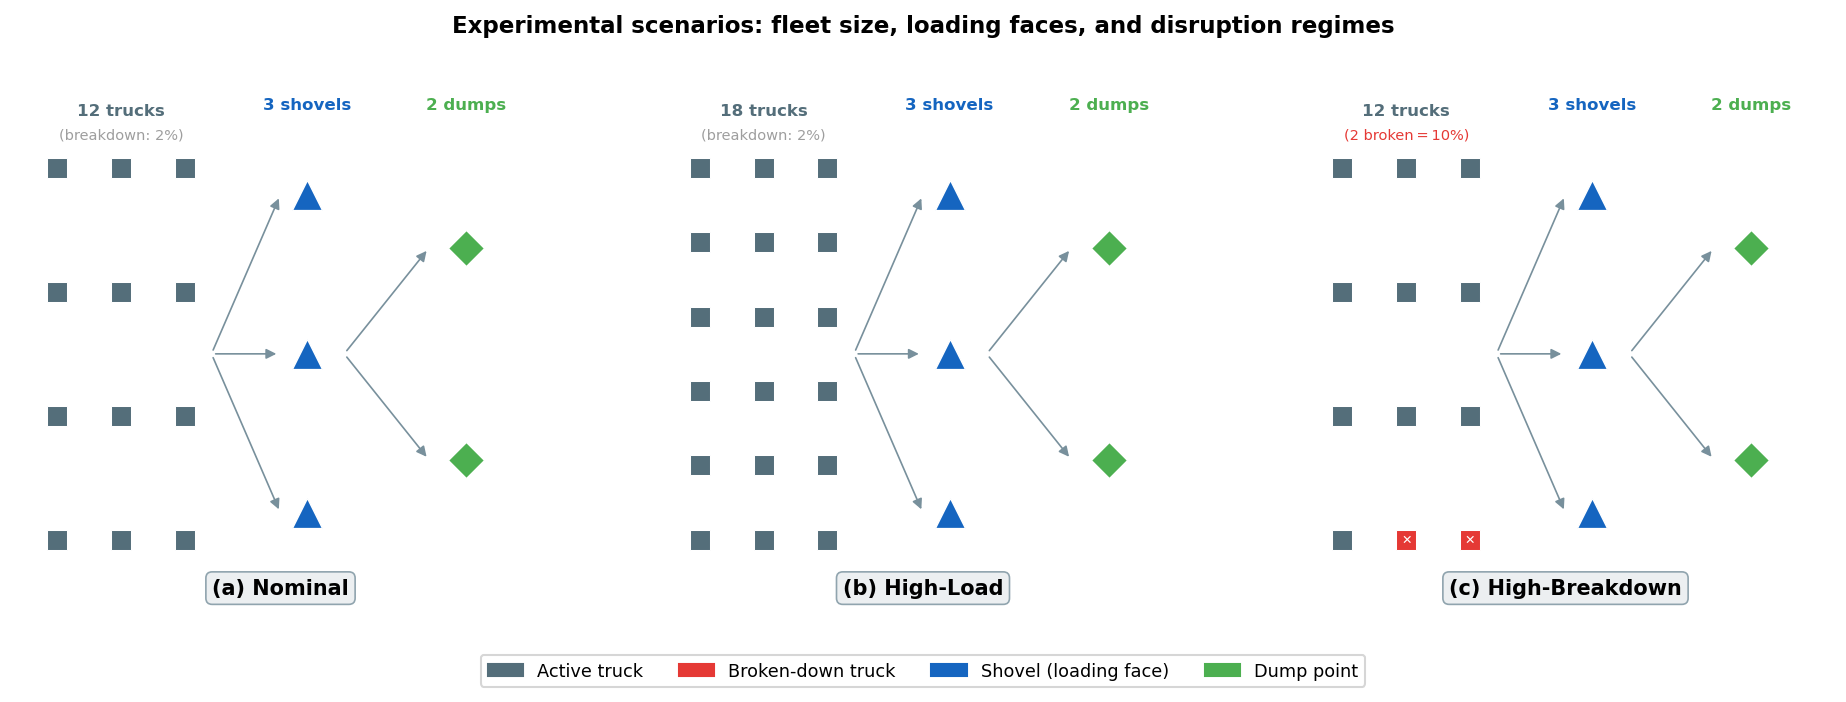
\includegraphics[width=0.95\textwidth]{figures/fig3_scenarios.png}
\caption{Configuration des trois scénarios expérimentaux.}
\label{fig:scenarios}
\end{figure}

\subsection{Références}

Afin d'établir un banc d'essai complet, l'agent PPO est comparé à sept autres politiques, regroupées en trois familles :

\begin{itemize}
  \item \textbf{Heuristiques statiques :} FIFO, Affectation fixe, Pelle la plus proche et Plus court chemin. Elles représentent les standards industriels actuels.
  \item \textbf{Apprentissage par renforcement tabulaire :} Q-Learning et SARSA, utilisés pour évaluer l'impact de l'approximation neuronale par rapport aux tables d'états discrètes.
  \item \textbf{Apprentissage par renforcement profond fondé sur la valeur :} DQN, utilisé pour opposer les méthodes de gradient de politique (PPO) à l'apprentissage profond fondé sur la valeur.
\end{itemize}

Pour la reproductibilité, les quatre heuristiques statiques sont définies précisément dans le \cref{tab:baselines}. Toutes sont évaluées exactement dans le même environnement, avec les mêmes graines aléatoires, que les agents d'apprentissage.

\begin{table}[H]
\centering
\caption{Définition formelle des heuristiques de dispatching statiques utilisées comme références.}
\label{tab:baselines}
\small
\begin{tabularx}{\textwidth}{lX}
\toprule
\textbf{Politique} & \textbf{Règle de décision appliquée lorsque le camion $i$ devient disponible} \\
\midrule
FIFO             & Affecter le camion $i$ à la pelle admissible dont la demande de chargement est en attente depuis le plus longtemps (égalités départagées par l'indice de la pelle). \\
Affectation fixe & Affecter le camion $i$ à la pelle $j(i)$ déterminée au début du poste ; la réaffectation n'a lieu que si $j(i)$ est indisponible (panne). \\
Pelle la plus proche & Affecter le camion $i$ à la pelle admissible minimisant la distance de trajet depuis la position courante du camion, sans tenir compte de la longueur de la file d'attente. \\
Plus court chemin & Affecter le camion $i$ à la destination admissible minimisant le temps de trajet attendu calculé par l'algorithme de Dijkstra sur le graphe routier courant. \\
\bottomrule
\end{tabularx}
\end{table}

\subsection{Métriques}
\label{sec:metrics}

Nous utilisons les indicateurs clés de performance (KPI) suivants pour évaluer l'efficacité de chaque politique :

\begin{enumerate}
  \item \textbf{Productivité :} tonnage total livré par heure (t/h).
  \item \textbf{Temps d'attente moyen :} durée moyenne pendant laquelle les camions restent inactifs en file d'attente par cycle (min).
  \item \textbf{Taux d'utilisation des équipements :} pourcentage du temps pendant lequel les pelles et les camions effectuent des tâches productives (\%).
  \item \textbf{Consommation spécifique :} carburant ou énergie consommé par tonne transportée, reflétant la durabilité (L/t). Les valeurs complètes inter-scénarios (les 8 politiques $\times$ 3 scénarios) sont rapportées dans le \cref{tab:efficiency} (\cref{sec:sustainability}).
  \item \textbf{Nombre de cycles terminés :} nombre total de cycles chargement--transport--déversement terminés pendant le poste. Rapporté pour les huit politiques dans les trois scénarios dans le \cref{tab:cycles_reward} (\cref{sec:results}).
  \item \textbf{Récompense cumulée :} la récompense totale accumulée sur l'épisode avec le vecteur de poids de référence ($w_1=1,\,w_2=0{,}1,\,w_3=0{,}05,\,w_4=0{,}3$). Comme toutes les politiques du banc d'essai principal sont évaluées avec les mêmes poids, les valeurs sont comparables entre elles ; elles sont rapportées dans le \cref{tab:cycles_reward}. La sensibilité de la récompense de PPO à $w_4$ seul est examinée plus avant dans l'étude d'ablation (\cref{tab:ablation}).
  \item \textbf{Ratio de robustesse :} pour quantifier la résilience, nous calculons le rapport entre la performance dans les scénarios perturbés et la performance en conditions nominales :
  \begin{equation}
  \mathrm{RR}(p,s) = \frac{\mathrm{Performance}(p,s)}{\mathrm{Performance}(p,\mathrm{nominal})} .
  \label{eq:rr}
  \end{equation}
\end{enumerate}

\subsection{Protocole statistique}
\label{sec:proto}

Conformément aux standards de la recherche à fort impact, nous ne nous appuyons pas sur des exécutions de simulation uniques.

\begin{itemize}
  \item \textbf{Réplications :} chaque politique est évaluée sur 30 réplications indépendantes afin de garantir la puissance statistique et la validité des intervalles de confiance.
  \item \textbf{Contrôle des graines aléatoires :} des graines aléatoires identiques sont utilisées pour toutes les politiques au sein de chaque réplication. Cela garantit que chaque algorithme est confronté exactement à la même séquence d'événements stochastiques (par exemple, une panne survient à la même minute pour PPO que pour FIFO).
  \item \textbf{Normalité et variance :} nous appliquons le test de Shapiro--Wilk pour vérifier la normalité et le test de Levene pour évaluer l'homogénéité des variances (homoscédasticité).
\end{itemize}

\paragraph{Statistiques inférentielles.} Selon le résultat des tests de normalité, nous appliquons :

\begin{itemize}
  \item \textbf{L'ANOVA à un facteur} (ou \textbf{l'ANOVA de Welch} en cas de variances inégales) pour déterminer s'il existe des différences significatives entre les politiques ; le test de \textbf{Kruskal--Wallis} est utilisé si l'hypothèse de normalité est violée.
  \item \textbf{Tests post-hoc :} tests $t$ de Welch par paires avec correction de Holm--Bonferroni (associés à l'ANOVA de Welch, car ils ne supposent pas l'homoscédasticité) ou test de Dunn fondé sur les rangs avec correction de Holm (associé à Kruskal--Wallis) afin d'identifier les différences par paires spécifiques. Le HSD de Tukey et Games--Howell sont délibérément écartés : tous deux exigent l'homoscédasticité ou une distribution de référence de l'étendue studentisée qui est inappropriée lorsque le test principal est celui de Kruskal--Wallis.
  \item \textbf{Correction de Holm--Bonferroni :} appliquée à toutes les valeurs $p$ afin de contrôler l'erreur de type I dans les comparaisons multiples.
  \item \textbf{Taille d'effet :} nous calculons le $d$ de Cohen (ou le $g$ de Hedges pour les petits échantillons) et le delta de Cliff pour mesurer l'ampleur pratique des améliorations de performance.
  \item \textbf{Intervalles de confiance :} des intervalles à 95\,\% sont générés par la méthode du bootstrap afin de fournir une plage robuste pour la performance moyenne.
\end{itemize}

\subsection{Paramètres de reproductibilité}

Pour garantir la reproductibilité de cette étude, tous les paramètres de simulation et hyperparamètres sont fixés. La simulation est implémentée en Python 3.11.11 avec Gymnasium 1.2.3 \cite{MarkTowers2025} et Stable-Baselines3 \cite{AntoninRaffin2021}. L'entraînement des agents PPO et DQN a été réalisé sur une configuration matérielle standardisée, tous les générateurs de nombres aléatoires (RNG) étant initialisés à partir d'une graine globale. Les poids de récompense spécifiques ($w_1 = 1$, $w_2 = 0{,}1$, $w_3 = 0{,}05$, $w_4 = 0{,}3$) ont été maintenus constants pendant toutes les expériences d'apprentissage par renforcement. Le code source, les fichiers de configuration et les listes de graines sont archivés dans le dépôt et décrits dans la section Disponibilité du code, de sorte que le protocole expérimental complet puisse être inspecté et réexécuté.

\paragraph{Protocole d'entraînement et d'évaluation.}
PPO et DQN ont été entraînés exclusivement sur le scénario nominal ($N=12$ camions, taux de panne~$=2\,\%$) pendant 2~millions de pas de temps d'environnement. Q-Learning et SARSA, dont l'unité naturelle de progression est l'épisode plutôt que l'interaction individuelle avec l'environnement, ont été entraînés pendant 30\,000 épisodes sur le même scénario (voir le Tableau~\ref{tab:hyper}) ; les deux budgets ne sont pas directement comparables en temps réel. Les agents profonds convergent dans leur budget ; les agents tabulaires non, de sorte que leur performance rapportée est une borne inférieure plutôt qu'un optimum convergé. L'évaluation sur les scénarios de forte charge et de fortes pannes a ensuite été réalisée en mode \textit{zero-shot} : les agents entraînés ont été déployés sans aucun ajustement fin supplémentaire, mesurant directement la généralisation hors distribution. Cette conception entraînement-sur-nominal / test-sur-perturbé est le fondement méthodologique des affirmations de résilience de la \cref{sec:results} : si les agents avaient été réentraînés par scénario, l'étude mesurerait l'adaptation, et non la robustesse.
% ============================================================================
% Section 6: Results
% ============================================================================
\section{Résultats}
\label{sec:results}

Cette section présente les résultats empiriques obtenus à partir de nos simulations multi-scénarios. Nous nous concentrons en particulier sur la hiérarchie de performance des politiques évaluées et sur l'évolution de leur comportement sous contrainte opérationnelle.

\subsection{Productivité}

L'indicateur de performance principal, la productivité en tonnes par heure, a été mesuré dans tous les scénarios. Le \cref{tab:productivity} rapporte les moyennes et les écarts-types des huit politiques, ainsi que la consommation spécifique de carburant en forte charge ; les valeurs complètes de carburant inter-scénarios figurent dans le \cref{tab:efficiency}.

\begin{table}[H]
\centering
\caption{Productivité moyenne (t/h), rapportée sous la forme moyenne $\pm$ écart-type sur 30 réplications.}
\label{tab:productivity}
\footnotesize\setlength{\tabcolsep}{3pt}
\begin{tabularx}{\textwidth}{@{}lXXXc@{}}
\toprule
\textbf{Politique} & \textbf{Nominal (t/h)} & \textbf{Forte charge (t/h)} & \textbf{Fortes pannes (t/h)} & \textbf{L/t} \\
\midrule
FIFO               & 3\,285,92 $\pm$ 41 & 4\,754,75 $\pm$ 63  & 3\,117,92 $\pm$ 62 & 0,0546 \\
Affectation fixe   & 4\,071,67 $\pm$ 43 & \textbf{5\,873,58 $\pm$ 76} & 3\,818,50 $\pm$ 67 & \textbf{0,0444} \\
Pelle la plus proche & 3\,824,92 $\pm$ 67 & 3\,948,00 $\pm$ 39  & 3\,661,58 $\pm$ 67 & 0,0582 \\
Plus court chemin  & 3\,868,08 $\pm$ 46 & 3\,962,00 $\pm$ 38  & 3\,692,50 $\pm$ 59 & 0,0588 \\
Q-Learning         & 3\,586,33 $\pm$ 99 & 4\,769,33 $\pm$ 102 & 3\,180,92 $\pm$ 92 & 0,0537 \\
SARSA              & 3\,085,25 $\pm$ 62 & 4\,044,83 $\pm$ 76  & 2\,980,83 $\pm$ 78 & 0,0612 \\
DQN (RL profond)   & 4\,134,67 $\pm$ 68 & 5\,651,33 $\pm$ 74  & \textbf{3\,949,17 $\pm$ 72} & 0,0445 \\
PPO (RL profond)   & \textbf{4\,176,67 $\pm$ 64} & 5\,149,08 $\pm$ 325 & 3\,899,58 $\pm$ 85 & 0,0475 \\
\bottomrule
\end{tabularx}
\end{table}

En conditions nominales, PPO a atteint la productivité la plus élevée (4\,176,67 t/h), surpassant l'Affectation fixe de 2,6\,\% et DQN (4\,134,67 t/h) de 1,0\,\% (\cref{fig:productivity}). Dans le scénario de fortes pannes, DQN s'est révélé le plus résilient (3\,949,17 t/h), tandis que PPO (3\,899,58 t/h) est resté légèrement en dessous. Dans le scénario de forte charge, l'Affectation fixe domine sur le débit brut (5\,873,58 t/h) et obtient simultanément le temps d'attente moyen le plus faible (43,2 min) ; DQN arrive juste derrière sur les deux indicateurs (5\,651,33 t/h, 47,8 min). Les heuristiques fondées sur la distance (Pelle la plus proche : 3\,948 t/h, 199,6 min ; Plus court chemin : 3\,962 t/h, 204,3 min) sont dominées au sens de Pareto sur les deux dimensions, ce qui étaye l'hypothèse H4. L'écart-type comparativement élevé de PPO en forte charge ($\pm$~325) reflète la variabilité d'une exécution à l'autre en cas de sursaturation de la flotte.

Le \cref{tab:cycles_reward} rapporte le nombre de cycles terminés et la récompense cumulée pour les mêmes exécutions. Comme toutes les politiques sont évaluées avec le même vecteur de poids, les valeurs de récompense sont comparables entre elles. Le classement selon la récompense cumulée coïncide avec le classement de productivité dans chaque scénario, ce qui confirme que la fonction de récompense incite efficacement au débit à l'échelle du système. L'effondrement marqué de la récompense de Pelle la plus proche et de Plus court chemin en forte charge, 161,4 et 160,5 contre plus de 200 pour les politiques fondées sur les files d'attente, reflète le terme de pénalité du temps d'attente $w_4 P_{\mathrm{wait}}$ et confirme empiriquement que la récompense multi-objectif pénalise la congestion.

\begin{figure}[H]
\centering
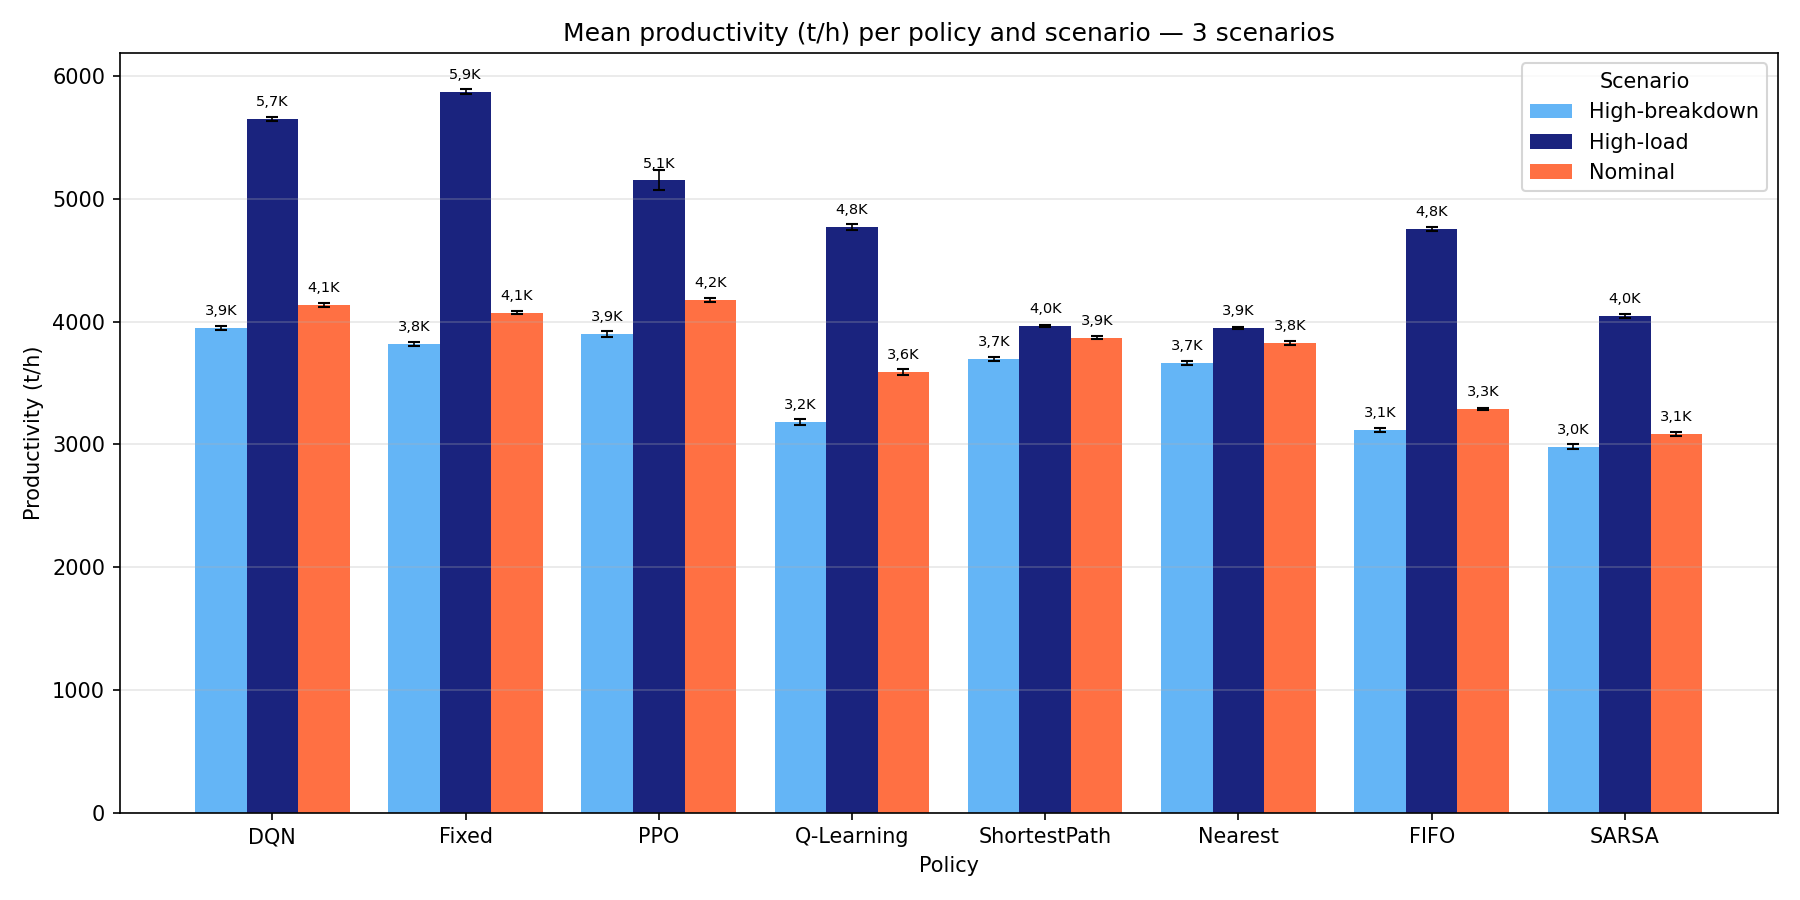
\includegraphics[width=0.92\textwidth]{figures/barplot_productivite_scenarios.png}
\caption{Productivité moyenne par politique et par scénario. Les barres d'erreur indiquent les intervalles de confiance bootstrap à 95\,\% sur les 30 réplications.}
\label{fig:productivity}
\end{figure}

\begin{table}[H]
\centering
\caption{Nombre moyen de cycles terminés et récompense cumulée par politique et par scénario, sur 30 réplications avec le vecteur de poids de référence (N : nominal, FC : forte charge, FP : fortes pannes).}
\label{tab:cycles_reward}
\small
\setlength{\tabcolsep}{4pt}
\renewcommand{\arraystretch}{1.05}
\begin{tabularx}{\textwidth}{@{}l*{6}{>{\centering\arraybackslash}X}@{}}
\toprule
\multirow{2}{*}{\textbf{Politique}}
  & \multicolumn{3}{c}{\textbf{Cycles terminés}}
  & \multicolumn{3}{c}{\textbf{Récompense cumulée}} \\
\cmidrule(lr){2-4}\cmidrule(lr){5-7}
  & \textbf{N} & \textbf{FC} & \textbf{FP}
  & \textbf{N}   & \textbf{FC}   & \textbf{FP} \\
\midrule
FIFO              & 187,8 & 271,7 & 178,2 & 163,1 & 234,0 & 155,0 \\
Affectation fixe  & 232,7 & \textbf{335,6} & 218,2 & 210,7 & \textbf{301,3} & 197,7 \\
Pelle la plus proche & 218,6 & 225,6 & 209,2 & 193,0 & 161,4 & 185,7 \\
Plus court chemin & 221,0 & 226,4 & 211,0 & 194,7 & 160,5 & 187,0 \\
Q-Learning        & 204,9 & 272,5 & 181,8 & 178,9 & 230,6 & 155,6 \\
SARSA             & 176,3 & 231,1 & 170,3 & 147,3 & 179,7 & 143,2 \\
DQN (RL profond)  & 236,3 & 322,9 & \textbf{225,7} & 213,8 & 288,9 & \textbf{204,4} \\
PPO (RL profond)  & \textbf{238,7} & 294,2 & 222,8 & \textbf{216,6} & 253,0 & 201,5 \\
\bottomrule
\end{tabularx}
\end{table}

\subsection{Temps d'attente et congestion}
\label{sec:waiting}

L'une des observations clés de cette étude est le découplage entre la productivité et la fluidité du système (\cref{fig:waiting,fig:pareto}). Dans le scénario de forte charge, bien que la productivité augmente en raison du nombre élevé de camions, la congestion devient le facteur limitant.

Nous avons observé un \textit{effondrement par congestion} propre aux heuristiques fondées sur la distance (Pelle la plus proche : $199{,}6 \pm 8{,}1$ min, Plus court chemin : $204{,}3 \pm 5{,}8$ min), où des camions concurrents saturent simultanément la même pelle. Les heuristiques fondées sur les files d'attente sont plus résilientes : FIFO ($45{,}2 \pm 4{,}0$ min) et Affectation fixe ($43{,}2 \pm 4{,}0$ min) gèrent la congestion presque aussi efficacement que DQN ($47{,}8 \pm 3{,}8$ min). PPO présente une variance plus élevée ($99{,}3 \pm 21{,}3$ min), reflétant des décisions d'acheminement occasionnellement sous-optimales en cas de saturation extrême de la flotte. Ces résultats indiquent que le \emph{type} de dispatching (fondé sur la distance, fondé sur les files d'attente ou appris) importe davantage que la distinction RL/non-RL pour l'indicateur de temps d'attente. Dans le scénario de fortes pannes, les agents DRL retrouvent une fluidité compétitive (PPO : 69,9~min ; DQN : 71,8~min), surpassant les méthodes tabulaires (SARSA : 81,8~min ; Q-Learning : 87,9~min) et les heuristiques fondées sur la distance ($\approx\!94$~min), bien que les heuristiques fondées sur les files d'attente conservent un avantage modéré (FIFO : 55,1~min ; Affectation fixe : 57,2~min). La \cref{fig:waiting} met en regard les trois politiques qui couvrent l'éventail des comportements observés : l'Affectation fixe et DQN restent en dessous de 50~min dans les trois scénarios, tandis que PPO atteint 99,3~min en cas de sursaturation de la flotte. La comparaison complète des huit politiques figure dans le \cref{tab:waiting}.

\begin{table}[H]
\centering
\caption{Temps d'attente moyen par cycle (minutes) $\pm$ écart-type sur 30 réplications.}
\label{tab:waiting}
\small
\begin{tabular}{lccc}
\toprule
\textbf{Politique} & \textbf{Nominal (min)} & \textbf{Forte charge (min)} & \textbf{Fortes pannes (min)} \\
\midrule
FIFO               & 33,5 $\pm$ 5,8  & 45,2 $\pm$ 4,0  & 55,1 $\pm$ 8,6  \\
Affectation fixe   & \textbf{29,4 $\pm$ 4,2}  & \textbf{43,2 $\pm$ 4,0}  & 57,2 $\pm$ 7,0  \\
Pelle la plus proche & 75,1 $\pm$ 6,4  & 199,6 $\pm$ 8,1 & 93,8 $\pm$ 7,1  \\
Plus court chemin  & 76,6 $\pm$ 6,1  & 204,3 $\pm$ 5,8 & 94,7 $\pm$ 6,5  \\
Q-Learning         & 58,1 $\pm$ 6,7  & 69,3 $\pm$ 3,9  & 87,9 $\pm$ 7,0  \\
SARSA              & 68,2 $\pm$ 5,8  & 119,9 $\pm$ 12,1 & 81,8 $\pm$ 8,4 \\
DQN (RL profond)   & 43,7 $\pm$ 5,2  & 47,8 $\pm$ 3,8  & 71,8 $\pm$ 6,2  \\
PPO (RL profond)   & 33,5 $\pm$ 4,8  & 99,3 $\pm$ 21,3 & \textbf{69,9 $\pm$ 8,0} \\
\bottomrule
\end{tabular}
\end{table}

\begin{figure}[H]
\centering
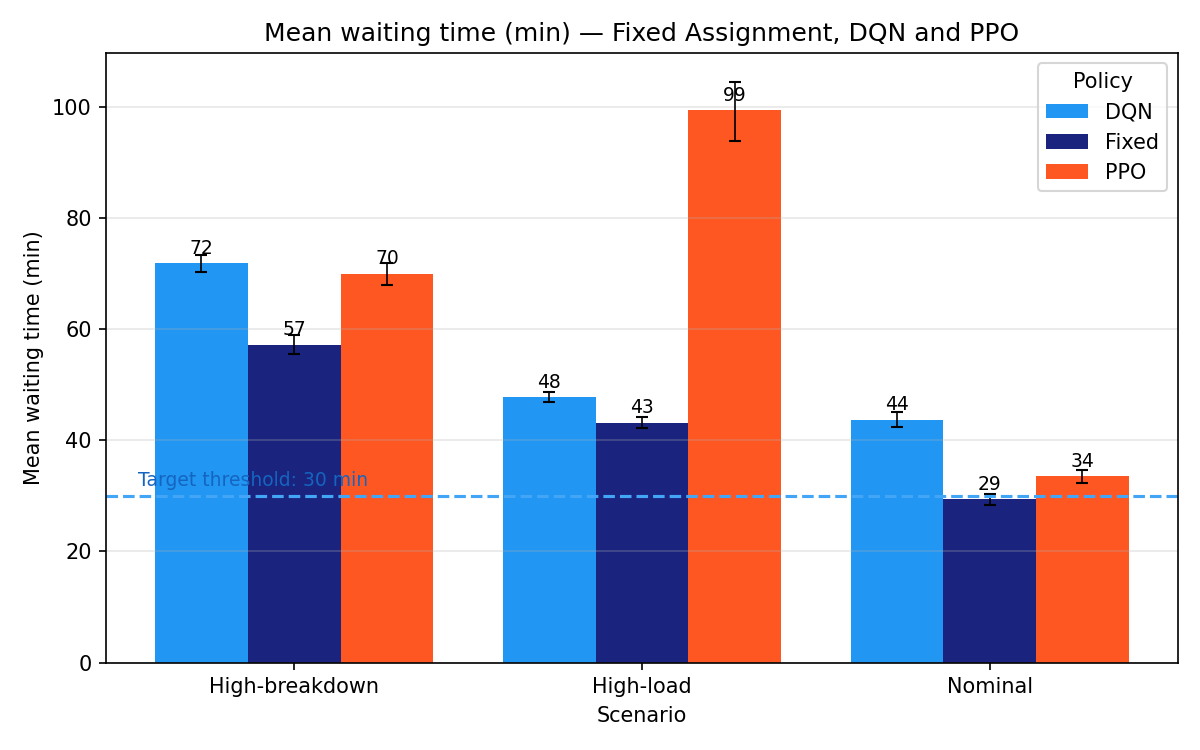
\includegraphics[width=0.92\textwidth]{figures/wait_time_comparison.png}
\caption{Temps d'attente moyen par cycle pour l'Affectation fixe, DQN et PPO. Les barres d'erreur indiquent les intervalles de confiance bootstrap à 95\,\%.}
\label{fig:waiting}
\end{figure}

La \cref{fig:pareto} place chaque couple (politique, scénario) dans le plan productivité--attente, de sorte que le coin inférieur droit correspond au comportement le plus souhaitable. Les points les plus performants appartiennent au scénario de forte charge plutôt qu'au scénario nominal : l'Affectation fixe atteint environ 5\,900~t/h pour 42~min et DQN environ 5\,600~t/h pour 47~min, car la flotte plus grande de 50\,\% produit un débit agrégé plus élevé tandis que les deux politiques maintiennent la congestion sous contrôle. Les heuristiques fondées sur la distance atteignent environ 200~min d'attente dans le même scénario, ce qui indique un régime de congestion sévère. Dans le scénario nominal, PPO et l'Affectation fixe forment le front de Pareto local, entre 4\,100 et 4\,200~t/h pour 29 à 34~min. Aucune politique unique n'occupe le front de Pareto global dans les trois régimes, ce qui confirme l'hypothèse~H4.

\begin{figure}[H]
\centering
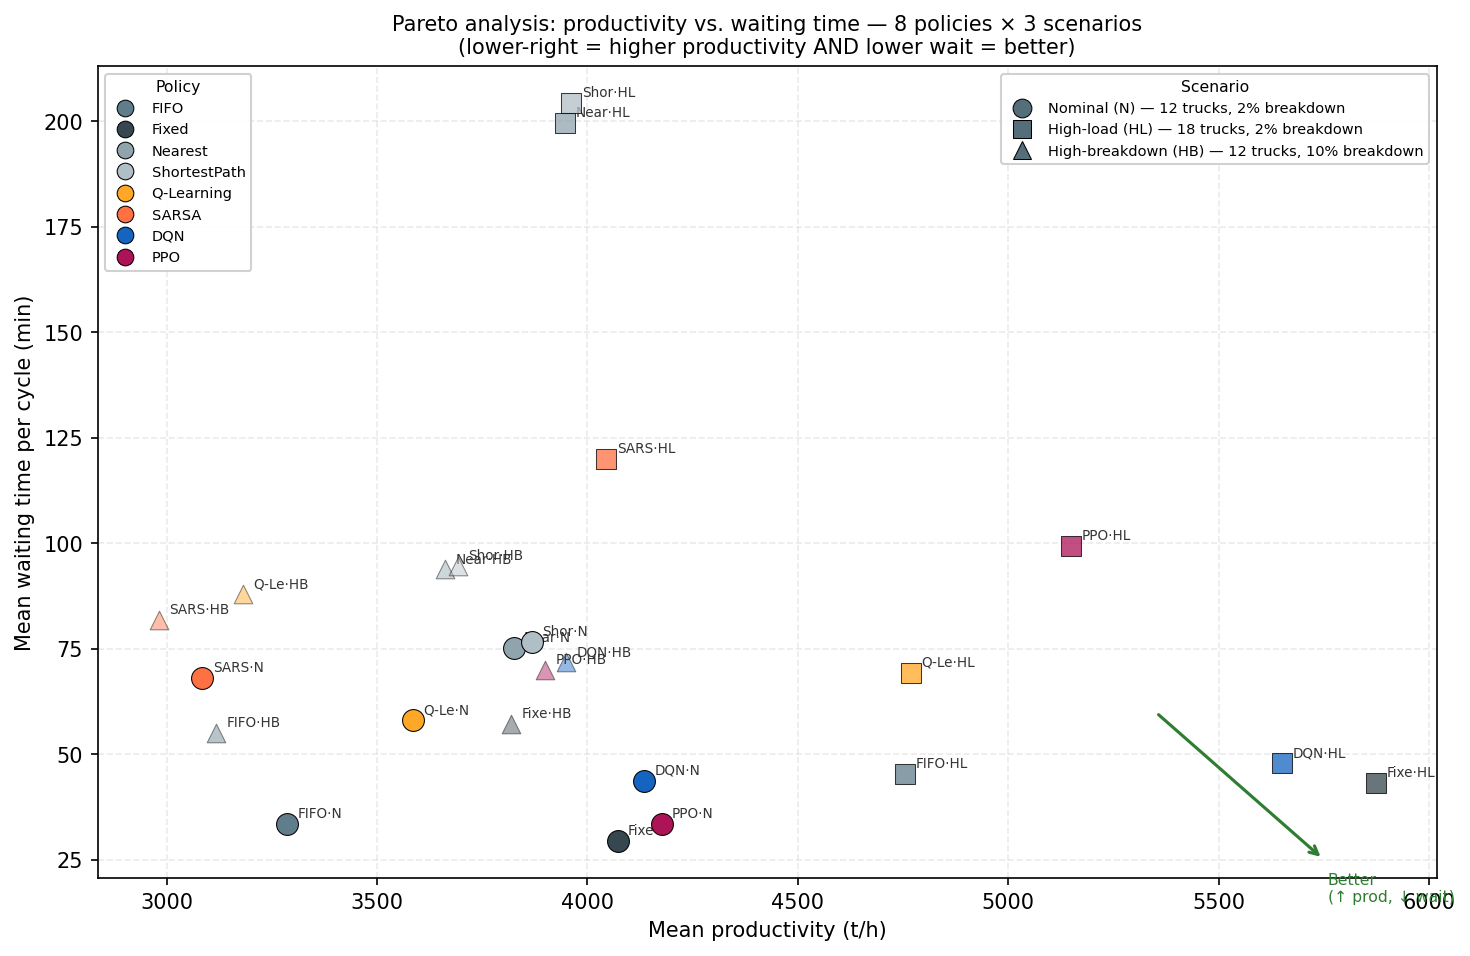
\includegraphics[width=0.88\textwidth]{figures/pareto_productivity_waiting.png}
\caption{Analyse de Pareto productivité--temps d'attente. La couleur désigne la politique et la forme du marqueur le scénario : cercle pour nominal, carré pour forte charge, triangle pour fortes pannes. Les étiquettes suivent la convention « Politique\textperiodcentered Scénario ».}
\label{fig:pareto}
\end{figure}

\subsection{Robustesse face aux perturbations}
\label{sec:robustness}

Cette analyse constitue le cœur scientifique du présent travail. Tous les agents RL ont été entraînés exclusivement sur le scénario nominal et évalués en mode \emph{zero-shot} sur les scénarios perturbés sans aucun ajustement fin supplémentaire ; les métriques ci-dessous mesurent donc la résilience hors distribution, et non la capacité d'adaptation.

Deux métriques de dégradation complémentaires sont introduites en plus du ratio de robustesse $\mathrm{RR}$ (\cref{eq:rr}). L'indice de dégradation en cas de panne $\Delta_{\mathrm{breakdown}}$ quantifie la part de productivité perdue lors du passage des conditions nominales aux conditions de fortes pannes :

\begin{equation}
\Delta_{\mathrm{breakdown}} = \frac{P_{\mathrm{nominal}} - P_{\mathrm{breakdown}}}{P_{\mathrm{nominal}}} \times 100 .
\label{eq:delta}
\end{equation}

\noindent L'indice d'augmentation du temps d'attente $\Delta_{\mathrm{wait}}^{s}$ capture la dégradation des files d'attente dans le scénario perturbé $s$ par rapport au nominal :

\begin{equation}
\Delta_{\mathrm{wait}}^{s} = \frac{W_{s} - W_{\mathrm{nominal}}}{W_{\mathrm{nominal}}} \times 100 .
\label{eq:delta_wait}
\end{equation}

\noindent Ensemble, ces deux indices fournissent un profil de résilience bidimensionnel : une dimension capture la capacité à maintenir le débit ; l'autre capture la capacité à contenir la formation de files d'attente sous contrainte. Le \cref{tab:robustness} rapporte le ratio de robustesse de productivité $\mathrm{RR}$, la dégradation du débit $\Delta_{\mathrm{breakdown}}$ de l'\cref{eq:delta}, et l'augmentation du temps d'attente de l'\cref{eq:delta_wait} mesurée en forte charge et en fortes pannes, toutes deux relativement au scénario nominal.

\begin{table}[H]
\centering
\caption{Analyse de robustesse multidimensionnelle pour toutes les politiques. Des valeurs de dégradation plus faibles indiquent une résilience plus élevée (FC : forte charge, FP : fortes pannes).}
\label{tab:robustness}
\small
\setlength{\tabcolsep}{4.5pt}
\begin{tabular}{l r r r r r}
\toprule
 & \multicolumn{2}{c}{\textbf{RR de productivité}} & \textbf{} & \multicolumn{2}{c}{\textbf{Augmentation du temps d'attente (\%)}} \\
\cmidrule(lr){2-3}\cmidrule(lr){5-6}
\textbf{Politique} & \textbf{RR(FC)} & \textbf{RR(FP)} & \textbf{$\Delta_{\mathrm{breakdown}}$ (\%)} & \textbf{$\Delta_{\mathrm{wait}}^{\mathrm{FC}}$} & \textbf{$\Delta_{\mathrm{wait}}^{\mathrm{FP}}$} \\
\midrule
FIFO               & 1,447 & 0,949 &  5,11  & +35,0  & +64,5  \\
Affectation fixe   & 1,443 & 0,938 &  6,22  & +47,0  & +94,8  \\
Pelle la plus proche & 1,032 & 0,957 &  4,27  & +165,9 & +24,9  \\
Plus court chemin  & 1,024 & 0,955 &  4,54  & +166,7 & +23,6  \\
Q-Learning         & 1,330 & 0,887 & 11,30  & +19,4  & +51,3  \\
SARSA              & 1,311 & \textbf{0,966} & \textbf{3,38} & +75,9 & \textbf{+20,0} \\
DQN (RL profond)   & 1,367 & 0,955 &  4,49  & \textbf{+9,3}  & +64,3  \\
PPO (RL profond)   & 1,233 & 0,934 &  6,63  & +196,4 & +108,7 \\
\bottomrule
\end{tabular}
\end{table}

\noindent\textbf{Dégradation du débit en cas de pannes d'équipements.} Sur l'axe de la productivité, l'ordre de dégradation en cas de panne est contre-intuitif. La stabilité \emph{relative} la plus élevée est affichée par SARSA ($\mathrm{RR}_{\mathrm{FP}}=0{,}966$, $\Delta=3{,}38\,\%$) et par les heuristiques fondées sur la distance (4,27\,\% et 4,54\,\%), mais cela reflète leurs références nominales déjà comprimées plutôt qu'une véritable résilience. La politique qui délivre le débit \emph{absolu} le plus élevé en cas de panne est DQN (3\,949,17~t/h, $\Delta=4{,}49\,\%$). PPO ($\Delta=6{,}63\,\%$) se dégrade davantage que DQN et FIFO (5,11\,\%), ce qui suggère que sa politique entraînée en nominal ne se transfère pas pleinement à des dynamiques perturbées. Q-Learning présente l'effondrement de productivité le plus important ($\Delta=11{,}30\,\%$), ce qui confirme que les fonctions de valeur tabulaires ne se généralisent pas aux chocs de panne discrets.

\noindent\textbf{Dégradation des files d'attente en cas de congestion de la flotte.} La dimension du temps d'attente révèle le résultat le plus frappant de cette étude. En forte charge, le temps d'attente de DQN n'augmente que de $\Delta_{\mathrm{wait}}^{\mathrm{FC}}=+9{,}3\,\%$, soit la politique la plus résiliente par une large marge. Le temps d'attente de PPO augmente de $+196{,}4\,\%$, la plus forte croissance de toutes les politiques malgré sa domination nominale. Les heuristiques fondées sur la distance s'effondrent également : Pelle la plus proche ($+165{,}9\,\%$) et Plus court chemin ($+166{,}7\,\%$) ne peuvent pas résoudre les demandes concurrentes sur des pelles chargées dès lors que la flotte dépasse la capacité d'absorption (voir la \cref{sec:waiting}). Les heuristiques fondées sur les files d'attente (FIFO $+35{,}0\,\%$, Affectation fixe $+47{,}0\,\%$) et Q-Learning ($+19{,}4\,\%$) restent relativement contenues. En fortes pannes, SARSA est de nouveau en tête sur la dimension du temps d'attente ($+20{,}0\,\%$), suivi de Pelle la plus proche et Plus court chemin ($+24{,}9\,\%$, $+23{,}6\,\%$) ; PPO enregistre la plus forte croissance absolue des files d'attente ($+108{,}7\,\%$), dépassant même l'Affectation fixe ($+94{,}8\,\%$).

\medskip
\noindent\textbf{Résultat central : découplage entre efficacité nominale et résilience opérationnelle.} Le \cref{tab:robustness} révèle une inversion systématique de la hiérarchie de performance d'un régime à l'autre. PPO, la politique la plus performante en conditions nominales (4\,176,67~t/h, 33,51~min d'attente), figure parmi les plus vulnérables tant en cas de congestion ($+196\,\%$ d'augmentation du temps d'attente) qu'en cas de panne ($\Delta=6{,}63\,\%$). DQN, deuxième en nominal, délivre le meilleur débit absolu en cas de panne et la réponse à la congestion la plus contenue (+9,3\,\%). Cette inversion démontre que la productivité nominale est un mauvais prédicteur de la résilience opérationnelle, et qu'une évaluation à régime unique aurait conduit à la conclusion erronée que PPO est la politique la plus déployable dans des environnements miniers variables. Dans la \cref{fig:heatmap}, le bloc supérieur rapporte la variation de productivité par rapport au nominal et le bloc inférieur la variation du temps d'attente, cette dernière sur une échelle inversée de sorte qu'une dégradation apparaît comme une valeur négative dans les deux blocs. Le contraste le plus marqué apparaît dans la colonne de forte charge, où le temps d'attente de PPO augmente de 196\,\% tandis que DQN reste stable à 9\,\%.

\begin{figure}[H]
\centering
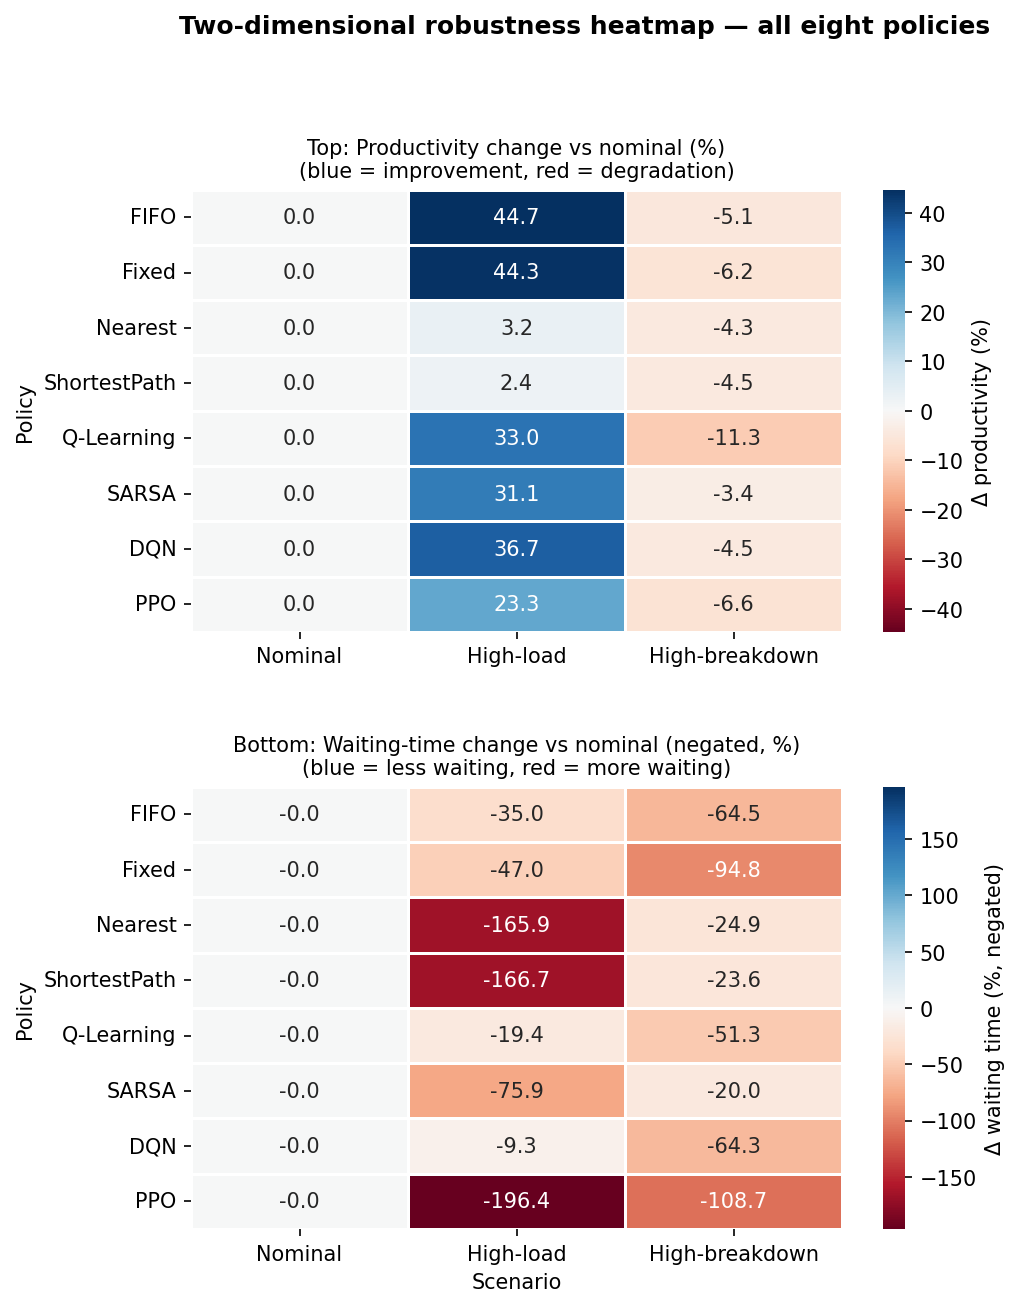
\includegraphics[width=0.9\textwidth]{figures/robustness_heatmap.png}
\caption{Carte thermique de robustesse des huit politiques dans les trois scénarios. Le bleu indique une amélioration par rapport au nominal et le rouge une dégradation ; le bloc du temps d'attente est tracé sur une échelle inversée de sorte que les deux blocs partagent le même sens de lecture.}
\label{fig:heatmap}
\end{figure}

\subsection{Significativité statistique}

Le choix du test suit les diagnostics distributionnels. En conditions nominales, Shapiro--Wilk rejette la normalité dans six des huit groupes et Levene détecte des variances hétérogènes ($p=2{,}3\times10^{-8}$) ; avec $n=30$ par groupe, le test $t$ de Welch reste valide en vertu du théorème central limite, de sorte qu'une analyse de variance de Welch est utilisée comme test omnibus et des tests $t$ de Welch par paires avec correction de Holm comme critère post-hoc. Dans les deux scénarios perturbés, au moins un groupe viole la normalité et les variances sont hétérogènes ; Kruskal--Wallis est donc utilisé comme test omnibus, avec le test post-hoc de Dunn fondé sur les rangs comme critère principal par paires. Les trois tests omnibus révèlent un effet significatif de la politique de dispatching sur la productivité ($p<0{,}001$).

Le test de Dunn est conservateur sous correction à nombreux groupes et ne détecte pas de différence significative à $\alpha=0{,}05$ pour trois comparaisons. Les tests $t$ de Welch correspondants donnent $p=5{,}2\times10^{-8}$ pour l'Affectation fixe contre DQN en forte charge, $p=2{,}7\times10^{-8}$ pour PPO contre l'Affectation fixe en fortes pannes, et $p=5{,}4\times10^{-4}$ pour DQN contre PPO dans le même scénario. Ces résultats paramétriques sont rapportés par souci d'exhaustivité ; le post-hoc de Dunn demeure le critère principal, conformément au cadre de Kruskal--Wallis. Les tailles d'effet et les intervalles de confiance à 95\,\% des différences de moyennes sont dérivés de tests $t$ de Welch par paires dans tous les scénarios. Le \cref{tab:stats} rapporte l'ensemble des résultats post-hoc par paires.

\begin{itemize}
  \item \textbf{Comparaisons par paires en nominal (Welch) :} PPO $>$ Affectation fixe ($p=4{,}01\times10^{-18}$, $d=1{,}942$, grand) ; DQN $>$ Affectation fixe ($p=2{,}13\times10^{-8}$, $d=1{,}112$, grand) ; PPO $>$ DQN ($p=3{,}21\times10^{-4}$, $d=0{,}640$, moyen).
  \item \textbf{Forte charge (Kruskal--Wallis, post-hoc de Dunn) :} l'Affectation fixe devance PPO ($p=1{,}27\times10^{-5}$, $d=3{,}096$, grand) et DQN ($p=0{,}062$, $d=3{,}004$ ; limite non significative après correction de Holm). Les politiques DRL ne surpassent pas l'heuristique statique sur le débit brut dans ce régime ; l'avantage de l'Affectation fixe sur DQN est numériquement important mais ne franchit pas le seuil corrigé.
  \item \textbf{Fortes pannes (Kruskal--Wallis, post-hoc de Dunn) :} DQN $>$ Affectation fixe ($p=5{,}78\times10^{-3}$, $d=1{,}896$, grand). PPO devance l'Affectation fixe de 81~t/h ($d=1{,}065$) mais le post-hoc fondé sur les rangs n'atteint pas la significativité ($p=0{,}144$) ; le test $t$ de Welch correspondant donne $p=2{,}7\times10^{-8}$, ce qui suggère que la différence est réelle mais atténuée par le caractère conservateur de la correction par rangs à nombreux groupes. DQN devance PPO de 49,6~t/h ($d=0{,}636$, Dunn $p=0{,}686$, Welch $p=5{,}4\times10^{-4}$) ; tout bien considéré, DQN est la politique de RL profond dominante en conditions de pannes.
\end{itemize}

\begin{table}[H]
\centering
\caption{Récapitulatif des tests statistiques sur la productivité (valeurs $p$ corrigées par Holm--Bonferroni).}
\label{tab:stats}
\scriptsize
\setlength{\tabcolsep}{3pt}
\begin{tabular}{llccc}
\toprule
\textbf{Scénario} & \textbf{Comparaison} & \textbf{Valeur $p$} & \textbf{Taille d'effet ($d$ de Cohen)} & \textbf{IC à 95\,\% de la différence} \\
\midrule
Nominal        & ANOVA de Welch (globale)      & $p < 0{,}001$, $F=3339$ & s.o. & s.o. \\
Nominal        & PPO vs Aff. fixe (Welch)  & $p=4{,}01\times10^{-18}$ & $d=1{,}942$ & $[85{,}4\,;\,124{,}6]$ \\
Nominal        & DQN vs Aff. fixe (Welch)  & $p=2{,}13\times10^{-8}$ & $d=1{,}112$ & $[42{,}5\,;\,83{,}5]$ \\
Nominal        & PPO vs DQN (Welch)          & $p=3{,}21\times10^{-4}$ & $d=0{,}640$ & $[18{,}3\,;\,65{,}7]$ \\
Forte charge   & Kruskal--Wallis              & $p < 0{,}001$, $H=445$            & s.o. & s.o. \\
Forte charge   & Aff. fixe vs DQN (Dunn)          & $p = 0{,}062$                     & $d=3{,}004$ & $[183{,}5\,;\,261{,}0]$ \\
Forte charge   & Aff. fixe vs PPO (Dunn)                & $p = 1{,}27\times10^{-5}$         & $d=3{,}096$ & $[600{,}4\,;\,848{,}6]$ \\
Fortes pannes  & Kruskal--Wallis              & $p < 0{,}001$, $H=437$            & s.o. & s.o. \\
Fortes pannes  & DQN vs Aff. fixe (Dunn)                & $p = 5{,}78\times10^{-3}$         & $d=1{,}896$ & $[105{,}7\,;\,155{,}6]$ \\
Fortes pannes  & PPO vs Aff. fixe (Dunn)          & $p = 0{,}144$                     & $d=1{,}065$ & $[53{,}5\,;\,108{,}6]$ \\
Fortes pannes  & DQN vs PPO (Dunn)            & $p = 0{,}686$                     & $d=0{,}636$ & $[21{,}4\,;\,77{,}8]$ \\
\bottomrule
\end{tabular}
\end{table}

\subsection{Stabilité inter-réplications}
\label{sec:stability}

Au-delà de la performance moyenne, une politique n'est déployable que si son comportement est reproductible d'un poste à l'autre. Nous calculons donc le coefficient de variation (CV\,=\,ET/moyenne) de la productivité sur les 30 réplications pour chaque politique et chaque scénario. Plus court chemin enregistre le CV moyen le plus faible sur les trois scénarios (1,25\,\%), bien que sa performance absolue figure parmi les plus basses, suivi de l'Affectation fixe (1,37\,\%), de FIFO et de Pelle la plus proche (1,52\,\% chacun). DQN est l'agent d'apprentissage le plus stable (1,59\,\%). À l'inverse, PPO présente la variabilité la plus élevée (3,34\,\%), due presque entièrement à ses réplications en forte charge (CV\,=\,6,31\,\%, ET\,=\,$\pm$\,325~t/h), où la sensibilité d'une exécution à l'autre aux décisions d'acheminement en cas de saturation de la flotte est prononcée. Les méthodes tabulaires présentent également une variabilité élevée (Q-Learning : 2,60\,\%, SARSA : 2,17\,\%), reflétant la sensibilité des fonctions de valeur discrétisées aux événements stochastiques. Pris conjointement avec le classement de productivité, l'Affectation fixe et DQN offrent la meilleure combinaison de haute performance et de faible variance inter-réplications, ce qui en fait les politiques les plus prévisibles pour un déploiement opérationnel.

\subsection{Convergence}

Les courbes d'entraînement des quatre agents d'apprentissage par renforcement, présentées dans la \cref{fig:convergence}, révèlent des comportements d'apprentissage distincts. Chaque courbe représente une seule exécution d'entraînement représentative, lissée par une moyenne mobile. Comme un entraînement multi-graines complet à 2~millions de pas de temps par agent est prohibitif en calcul, les bandes de confiance sur les trajectoires d'entraînement ne sont pas rapportées ici ; la robustesse statistique des estimations de performance finales est établie par le protocole d'évaluation à 30 réplications décrit dans la \cref{sec:proto} et reflétée dans les intervalles de confiance du \cref{tab:productivity}.

\begin{itemize}
  \item \textbf{Agents RL profonds :} PPO et DQN affichent une convergence stable en moins de 2~millions de pas. La productivité de PPO augmente de façon monotone et atteint un plateau autour de 4\,000--4\,200~t/h ; DQN présente des oscillations initiales plus importantes attribuables à son exploration $\varepsilon$-greedy, avant de se stabiliser à un niveau similaire. La variance du signal de récompense diminue progressivement au fil de l'entraînement, ce qui indique que les deux agents identifient des stratégies d'affectation robustes.
  \item \textbf{Agents tabulaires :} les deux agents tabulaires se comportent différemment sur le budget de 30\,000 épisodes. Q-Learning reste stable pendant environ 12\,000 épisodes, puis s'améliore régulièrement jusqu'à la fin du budget sans atteindre de plateau, de sorte que sa performance rapportée doit être lue comme une borne inférieure de ce que la méthode pourrait atteindre avec un budget plus long. SARSA ne montre aucune amélioration mesurable sur le même budget, ce qui est cohérent avec sa faible productivité finale (3\,085~t/h en nominal, \cref{tab:productivity}). Ces deux résultats indiquent qu'une représentation discrète avec $n_{\text{bins}}=8$ par dimension ne peut pas capturer les interdépendances de grande dimension d'un environnement multi-pelles à 12 camions dans un budget d'épisodes réaliste.
\end{itemize}

Les agents profonds et tabulaires sont tracés sur des panneaux séparés dans la \cref{fig:convergence} car ils sont enregistrés sur des grandeurs différentes : les agents profonds sur la productivité en tonnes par heure, les agents tabulaires sur la récompense cumulée par épisode. Les panneaux ne sont donc pas directement comparables en amplitude, et seule la forme de chaque trajectoire doit être lue d'un panneau à l'autre.

\begin{figure}[H]
\centering
\begin{subfigure}[b]{0.49\textwidth}
  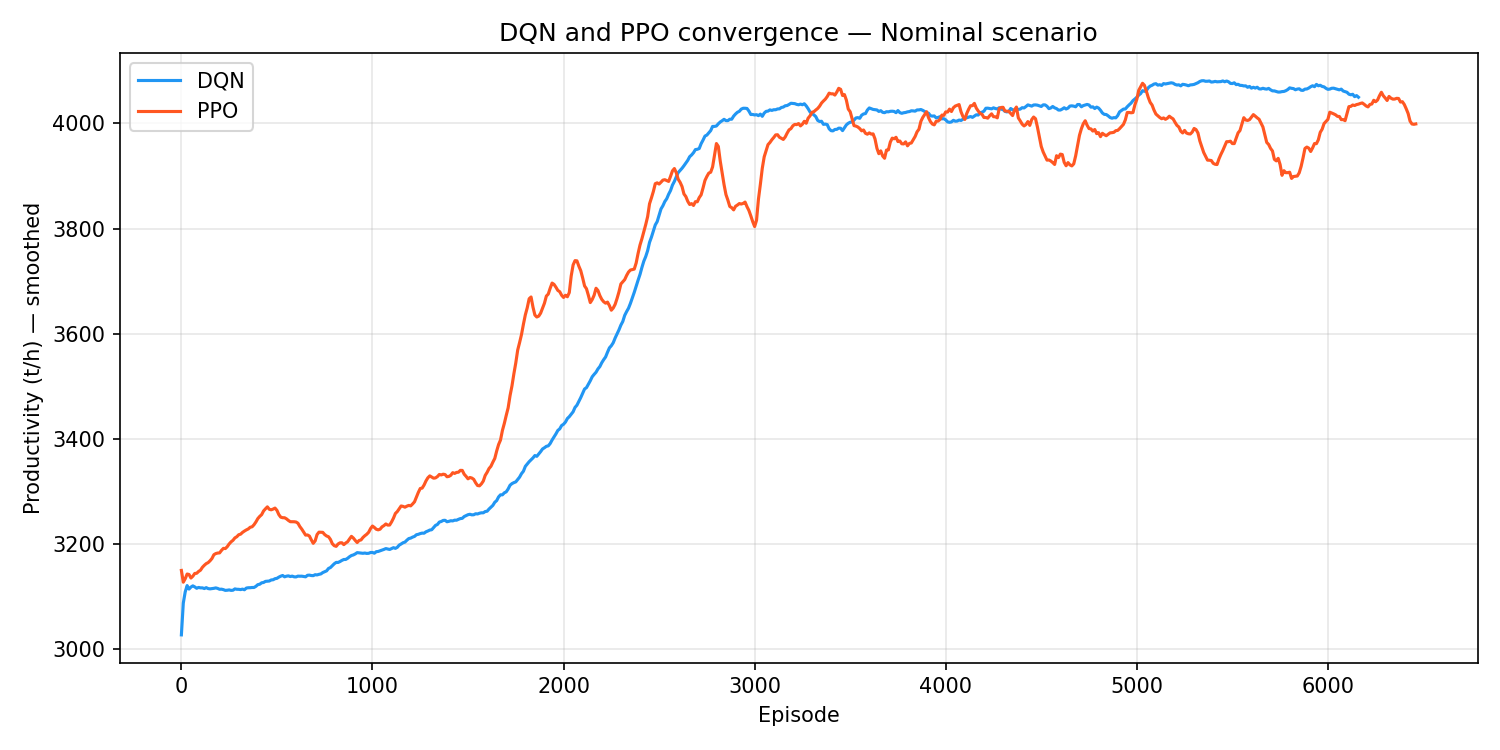
\includegraphics[width=\textwidth]{figures/learning_curves_deeprl_nominal.png}
  \caption{Agents RL profonds (DQN, PPO), scénario nominal}
\end{subfigure}
\hfill
\begin{subfigure}[b]{0.49\textwidth}
  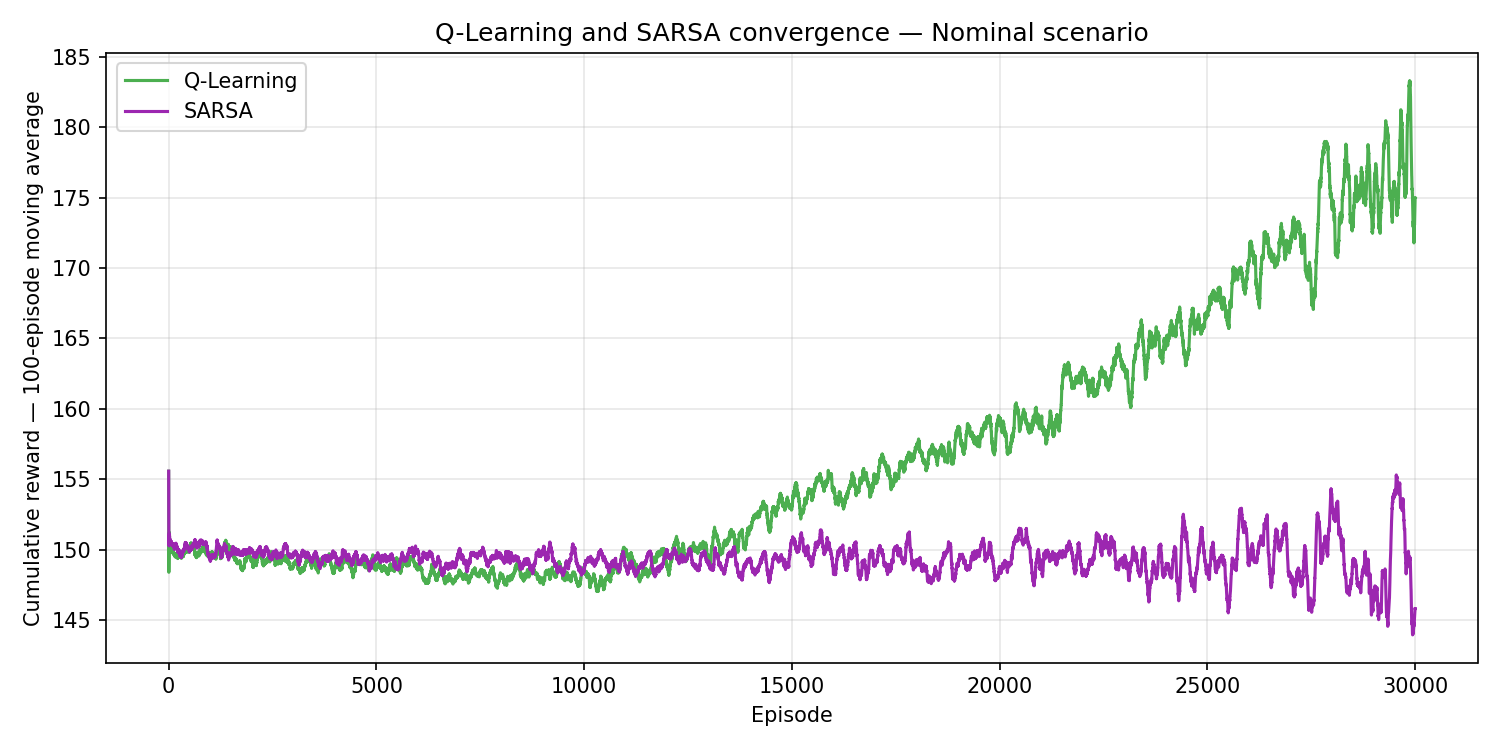
\includegraphics[width=\textwidth]{figures/learning_curves_nominal.png}
  \caption{Agents tabulaires (Q-Learning, SARSA), scénario nominal}
\end{subfigure}
\caption{Courbes d'entraînement sur le scénario nominal, exécution unique représentative. Gauche : productivité des agents profonds en tonnes par heure. Droite : récompense cumulée par épisode des agents tabulaires, moyenne mobile sur 100 épisodes.}
\label{fig:convergence}
\end{figure}

\subsection{Étude d'ablation}
\label{sec:ablation}

L'étude d'ablation porte sur le poids de la pénalité de temps d'attente ($w_4$) dans la fonction de récompense, tous les autres poids étant maintenus constants ($w_1 = 1$, $w_2 = 0{,}1$, $w_3 = 0{,}05$). Pour chaque valeur de $w_4$, un seul modèle PPO a été entraîné à partir de zéro ; la moyenne et l'écart-type rapportés sont calculés sur 30 épisodes d'évaluation indépendants de ce modèle entraîné, chacun avec une graine aléatoire différente. L'écart-type reflète donc la variabilité d'évaluation sous stochasticité de la simulation plutôt que la variance d'entraînement ; des conclusions sur la stabilité de l'entraînement exigeraient plusieurs entraînements indépendants.

Les résultats révèlent une relation non monotone entre $w_4$ et la performance. Lorsque $w_4 = 0$, l'agent atteint 4\,160,9~t/h avec 41,5~min de temps d'attente : la productivité est marginalement inférieure à la référence ($-0{,}4\,\%$) mais les temps d'attente augmentent de 23,9\,\%. Le résultat surprenant se situe à $w_4 = 0{,}1$ : une pénalité faible mais non nulle donne les \emph{pires} résultats simultanément sur les deux métriques (3\,931,7~t/h, $-5{,}9\,\%$ ; 74,8~min, $+123\,\%$). Cela suggère qu'une pénalité insuffisamment pondérée introduit des signaux de gradient conflictuels pendant l'entraînement, amenant la politique à converger vers un équilibre sous-optimal plutôt que vers une stratégie cohérente. À $w_4 = 0{,}3$, l'agent atteint le meilleur compromis (4\,176,7~t/h, 33,5~min), confirmant qu'une pénalité d'attente bien calibrée oriente la politique vers un flux à l'échelle du système sans sacrifier le débit. Avec $w_4 = 0{,}5$, une pénalité trop conservatrice inverse le gain : la productivité s'effondre à 3\,683,8~t/h ($-11{,}8\,\%$), le temps d'attente monte à 79,3~min ($+137\,\%$) et le taux d'utilisation des équipements tombe à 83,7\,\%, le plus bas de toutes les configurations. L'écart-type notablement plus grand ($\pm$~158~t/h) reflète une variance d'évaluation plus élevée sous cette configuration, ce qui suggère que la politique entraînée produit des décisions d'acheminement incohérentes d'une exécution de simulation stochastique à l'autre. Ces résultats soulignent la sensibilité de l'ingénierie de la récompense en apprentissage par renforcement multi-objectif : le choix de $w_4$ n'est pas un simple curseur, mais un paramètre de conception critique aux effets non monotones sur la convergence de la politique ; une valeur intermédiaire bien calibrée ($w_4 = 0{,}3$) est essentielle pour obtenir une optimisation cohérente à l'échelle du système. Dans le \cref{tab:ablation}, chaque ligne est évaluée avec sa propre valeur de $w_4$, de sorte que la colonne de récompense cumulée n'est pas directement comparable d'une ligne à l'autre.

\begin{table}[H]
\centering
\caption{Étude d'ablation sur le poids de la pénalité de temps d'attente $w_4$, scénario nominal. Les valeurs sont rapportées sous la forme moyenne $\pm$ écart-type sur 30 exécutions d'évaluation ; chaque ligne est évaluée avec son propre $w_4$, de sorte que la colonne de récompense n'est pas comparable d'une ligne à l'autre.}
\label{tab:ablation}
\small
\begin{tabular}{lcccc}
\toprule
\textbf{$w_4$} & \textbf{Productivité (t/h)} & \textbf{Temps d'attente (min)} & \textbf{Utilisation (\%)} & \textbf{Récomp. cum.} \\
\midrule
0,0  & 4\,160,9 $\pm$ 64 & 41,5 $\pm$ 4,8 & 94,3 & 218,4 \\
0,1  & 3\,931,7 $\pm$ 52 & 74,8 $\pm$ 4,6 & 84,5 & 205,1 \\
0,3 (réf.) & \textbf{4\,176,7 $\pm$ 64} & \textbf{33,5 $\pm$ 4,8} & \textbf{94,5} & 216,6 \\
0,5  & 3\,683,8 $\pm$ 158 & 79,3 $\pm$ 20,3 & 83,7 & 178,9 \\
\bottomrule
\end{tabular}

\end{table}

\paragraph{Sensibilité aux hyperparamètres.}
La configuration PPO de référence ($\alpha = 3 \times 10^{-4}$,
$c_H = 0{,}02$, $\varepsilon_{\text{clip}} = 0{,}2$,
$n_{\text{steps}} = 1024$, $n_{\text{epochs}} = 10$) suit les
réglages canoniques de~\cite{JohnSchulman2017}.
Un balayage de sensibilité qualitatif préliminaire a été mené avant la configuration finale :
(i)~la variation du coefficient d'entropie sur $c_H \in \{0{,}0\,;\, 0{,}01\,;\, 0{,}02\,;\, 0{,}05\}$
a indiqué que $c_H = 0{,}02$ offrait le meilleur compromis de convergence observé, car des valeurs plus faibles produisaient une convergence prématurée vers des itinéraires de dispatching localement optimaux,
tandis que des valeurs plus élevées retardaient la convergence sans amélioration visible de la productivité finale ;
(ii)~des taux d'apprentissage en dehors de $[10^{-4},\, 10^{-3}]$ entraînaient soit une convergence lente
soit des courbes de récompense oscillantes ;
(iii)~la plage d'écrêtage $\varepsilon_{\text{clip}} = 0{,}2$ est la valeur par défaut canonique~\cite{JohnSchulman2017}
et est apparue insensible dans ce cadre à actions discrètes.
Ces observations qualitatives soutiennent la configuration choisie comme point de départ raisonnable ; un rapport formel de recherche par grille est laissé à des travaux futurs.

% ============================================================================
% Section 7: Discussion
% ============================================================================
\section{Discussion}
\label{sec:discussion}

Cette section interprète les résultats expérimentaux au regard des questions de recherche et de la dépendance du classement des politiques au régime. Elle discute l'inversion entre efficacité nominale et résilience opérationnelle, le mécanisme de congestion propre aux règles fondées sur la distance, les implications industrielles de ces résultats et les limites de l'étude.

Les expériences répondent à la QR1 en montrant qu'aucune politique unique n'atteint la productivité la plus élevée dans chaque scénario. PPO est en tête en conditions nominales (4\,176,7~t/h), l'Affectation fixe en cas de sursaturation de la flotte (5\,873,6~t/h) et DQN en cas de pannes d'équipements fréquentes (3\,949,2~t/h). Le classement n'est donc pas une propriété de la famille d'algorithmes mais de l'interaction entre la logique de dispatching et le régime de fonctionnement, ce qui est le résultat central de cette étude.

Concernant la QR2, le compromis entre productivité et temps d'attente dépend lui-même du régime. En conditions nominales, les deux objectifs sont globalement alignés : les politiques qui déplacent le plus de matériau sont aussi celles qui font le moins la queue, et PPO et l'Affectation fixe forment un front de Pareto local. En cas de sursaturation de la flotte, les deux objectifs se séparent nettement, puisque Pelle la plus proche et Plus court chemin combinent le débit le plus faible avec des temps d'attente proches de 200~min, tandis que l'Affectation fixe et DQN s'améliorent simultanément sur les deux dimensions. Le découplage n'est donc pas une propriété générale du dispatching, mais la conséquence de la manière dont une règle donnée résout les demandes concurrentes une fois que la demande dépasse la capacité de chargement.

Pour la QR3, les écarts observés survivent inégalement à la correction. En conditions nominales, les trois comparaisons par paires d'intérêt restent significatives après correction de Holm, avec de grandes tailles d'effet. Dans les deux scénarios perturbés, le post-hoc de Dunn fondé sur les rangs est nettement plus conservateur : l'avantage de l'Affectation fixe sur DQN en forte charge ($p=0{,}062$) et celui de DQN sur PPO en fortes pannes ($p=0{,}686$) ne franchissent pas le seuil, bien que les tests de Welch correspondants et les tailles d'effet indiquent une différence réelle. Ne rapporter que les résultats paramétriques aurait donc surestimé les preuves, c'est pourquoi le post-hoc de Dunn est conservé comme critère principal.

La QR4 reçoit une réponse nuancée. Les agents profonds ne se dégradent pas uniformément moins que les règles statiques lorsqu'ils sont déployés sur des régimes pour lesquels ils n'ont pas été entraînés. Sur le débit, PPO perd 6,63\,\% en cas de panne, plus que FIFO (5,11\,\%) et plus que DQN (4,49\,\%). Sur la formation des files d'attente, DQN est la politique la plus résiliente du banc d'essai en cas de sursaturation de la flotte ($+9{,}3\,\%$), tandis que PPO enregistre la plus forte détérioration de toutes les politiques ($+196{,}4\,\%$). La robustesse \textit{zero-shot} est donc une propriété de l'agent individuel plutôt que de la famille de l'apprentissage par renforcement profond dans son ensemble, et elle ne découle pas de la performance nominale.

La QR5 sépare la performance moyenne de la prévisibilité. L'Affectation fixe et DQN combinent un débit élevé et une faible variance inter-réplications, tandis que PPO est la politique la moins prévisible du banc d'essai, presque entièrement en raison de son comportement en cas de sursaturation de la flotte. Pour un exploitant, une politique dont la production fluctue de plus de six pour cent d'un poste à l'autre est plus difficile à planifier qu'une alternative légèrement moins productive mais plus régulière, ce qui constitue un argument pratique que la seule productivité moyenne ne capture pas.

La QR6 montre que le classement sur la consommation spécifique de carburant ne suit pas le classement de productivité. DQN, deuxième en débit nominal, obtient la consommation par tonne la plus faible dans deux des trois scénarios, tandis que PPO, premier en débit nominal, consomme davantage que l'Affectation fixe en cas de sursaturation de la flotte. L'efficacité énergétique est donc une troisième dimension aux côtés du débit et de la fluidité, et elle réordonne une fois de plus les politiques.

Le \cref{tab:hypotheses} résume le statut de validation des quatre hypothèses énoncées dans la \cref{sec:rq}.

\begin{table}[H]
\caption{Validation des quatre hypothèses de recherche au regard des résultats empiriques.}
\label{tab:hypotheses}
\footnotesize\setlength{\tabcolsep}{4pt}
\begin{tabularx}{\textwidth}{@{}lXXl@{}}
\toprule
\textbf{Hyp.} & \textbf{Énoncé} & \textbf{Preuves clés} & \textbf{Verdict} \\
\midrule
H1 & DRL $>$ heuristiques en productivité en conditions nominales. & PPO est en tête en nominal (4\,176,7~t/h, $+2{,}6\,\%$ vs Affectation fixe, $p<0{,}001$, $d=1{,}94$) ; DQN second (4\,134,7~t/h, $+1{,}6\,\%$ vs Aff. fixe, $p<0{,}001$, $d=1{,}11$). Les deux agents DRL surpassent les quatre heuristiques statiques. & \textbf{Validée} \\[4pt]
H2 & Le DRL présente une moindre dégradation en cas de perturbations. & Sur le tonnage : PPO $\Delta{=}6{,}63\,\%$ vs FIFO $5{,}11\,\%$, ce qui \textit{réfute} l'énoncé (le DRL se dégrade davantage). Sur le temps d'attente : en forte charge, DQN (47,8 min) et Q-Learning (69,3 min) surpassent les heuristiques fondées sur la distance (Pelle la plus proche 199,6, PCC 204,3 min) ; les heuristiques fondées sur les files d'attente (FIFO 45,2, Aff. fixe 43,2 min) sont comparables à DQN. En fortes pannes, le RL profond (PPO 69,9 min, DQN 71,8 min) surpasse également le RL tabulaire (SARSA 81,8, Q-Learning 87,9) et les heuristiques fondées sur la distance ($\approx$94 min), mais pas les heuristiques fondées sur les files d'attente (FIFO 55,1, Aff. fixe 57,2 min). & Partiellement validée \\[4pt]
H3 & Aucune politique unique ne domine dans tous les régimes. & PPO meilleur en nominal ; DQN meilleur en fortes pannes ; Aff. fixe meilleure en forte charge (tonnage brut et fluidité simultanément). & \textbf{Validée} \\[4pt]
H4 & Productivité élevée $\not\Rightarrow$ faible congestion. & Pelle la plus proche et Plus court chemin illustrent le découplage : faible productivité ($\approx$3\,950 t/h) ET congestion sévère ($\approx$200 min : Pelle la plus proche 199,6, PCC 204,3), dominées sur les deux métriques par l'Aff. fixe (5\,874 t/h, 43,2 min) et DQN (5\,651 t/h, 47,8 min). Le \emph{type} de dispatching (fondé sur la distance vs fondé sur les files d'attente vs appris) détermine le résultat productivité--fluidité. & \textbf{Validée} \\
\bottomrule
\end{tabularx}
\end{table}

\subsection{Interprétation scientifique}

L'une des principales conclusions de cette recherche est qu'aucune politique de dispatching n'est universellement dominante.

\begin{itemize}
  \item \textbf{PPO vs DQN :} la supériorité de PPO en conditions nominales (4\,176,67 t/h vs DQN 4\,135 t/h, $d=0{,}640$) peut être attribuée à sa nature de gradient de politique, qui permet une exploration plus fluide dans des espaces d'états de grande dimension. DQN atteint le meilleur débit absolu en fortes pannes (3\,949 t/h), devançant PPO de 49,6~t/h ($d=0{,}636$, IC à 95\,\% $[21{,}4\,;\,77{,}8]$~t/h ; Welch $p=5{,}4\times10^{-4}$, post-hoc de Dunn $p=0{,}686$). Le tampon de rejeu d'expériences de DQN permet à l'agent de réutiliser les états de transition impliquant des pannes d'équipements sur plusieurs mises à jour du gradient, ce qui peut contribuer à sa robustesse en conditions de pannes, un mécanisme indisponible pour l'agent PPO on-policy.
  \item \textbf{Le DRL comme agent de pilotage de la charge en temps réel :} les heuristiques fondées sur la distance telles que Pelle la plus proche créent des « points chauds » en acheminant chaque camion disponible vers l'excavatrice physiquement la plus proche, quel que soit l'état de sa file d'attente. En cas de sursaturation de la flotte, cela produit une cascade de congestion : Pelle la plus proche atteint 199,6~min de temps d'attente moyen en forte charge contre 43,2~min pour l'Affectation fixe (\cref{tab:waiting}). Les agents DRL évitent cela en apprenant à équilibrer la pression des files d'attente entre les pelles à chaque point de décision. La \cref{fig:behavioral} fournit une preuve empirique directe : le panneau~(C) compare l'entropie d'affectation de Pelle la plus proche et de PPO sur un épisode de forte charge de 480 min. L'entropie de Pelle la plus proche s'effondre à $H\approx 0$ dès les premiers cycles. Les 18 camions convergent tous vers la même excavatrice géographiquement la plus proche, laissant les deux autres inactives et créant le point chaud persistant visible dans le panneau~(A). PPO, en revanche, maintient une entropie plus élevée et plus stable, répartissant le trafic entre les trois pelles (panneau~B). Cette allocation plus large divise par deux l'arriéré moyen des files d'attente, ce qui indique que l'avantage de PPO en temps d'attente en forte charge (99,3~min contre 199,6~min pour Pelle la plus proche, soit une réduction de 50\,\%) est dû à la différence d'entropie plutôt qu'à un choix fortuit de paramètres.
  \item \textbf{Découplage entre efficacité nominale et résilience opérationnelle :} le \cref{tab:robustness} quantifie une inversion systématique de la hiérarchie de performance d'un régime opérationnel à l'autre. PPO, la politique la plus performante en productivité nominale (4\,176,67~t/h), enregistre la plus forte détérioration du temps d'attente en cas de congestion de la flotte ($\Delta_{\mathrm{wait}}^{\mathrm{FC}}=+196{,}4\,\%$) et une dégradation du débit ($\Delta=6{,}63\,\%$) supérieure à celle de FIFO ($5{,}11\,\%$) et de DQN ($4{,}49\,\%$) en fortes pannes. DQN présente le profil opposé : deuxième en productivité nominale, meilleur débit absolu en cas de panne (3\,949,17~t/h) et plus résilient à la congestion ($\Delta_{\mathrm{wait}}^{\mathrm{FC}}=+9{,}3\,\%$). Ce résultat a une implication méthodologique directe : une évaluation menée sur le seul scénario nominal classerait PPO comme la politique la plus déployable, alors qu'une évaluation multi-régimes révèle que DQN offre une résilience opérationnelle supérieure dans les deux régimes perturbés. Les bancs d'essai de FMS miniers devraient donc être évalués sur au moins deux types de perturbation contrastés avant que des recommandations opérationnelles ne soient formulées.
  \item \textbf{Un problème stochastique et multi-objectif :} le découplage entre tonnage et temps d'attente observé dans le scénario de forte charge étaye l'hypothèse H4 et confirme que le dispatching minier doit être traité comme un problème de décision véritablement multi-objectif et stochastique plutôt que comme une maximisation du débit à critère unique.
\end{itemize}

\begin{figure}[H]
\centering
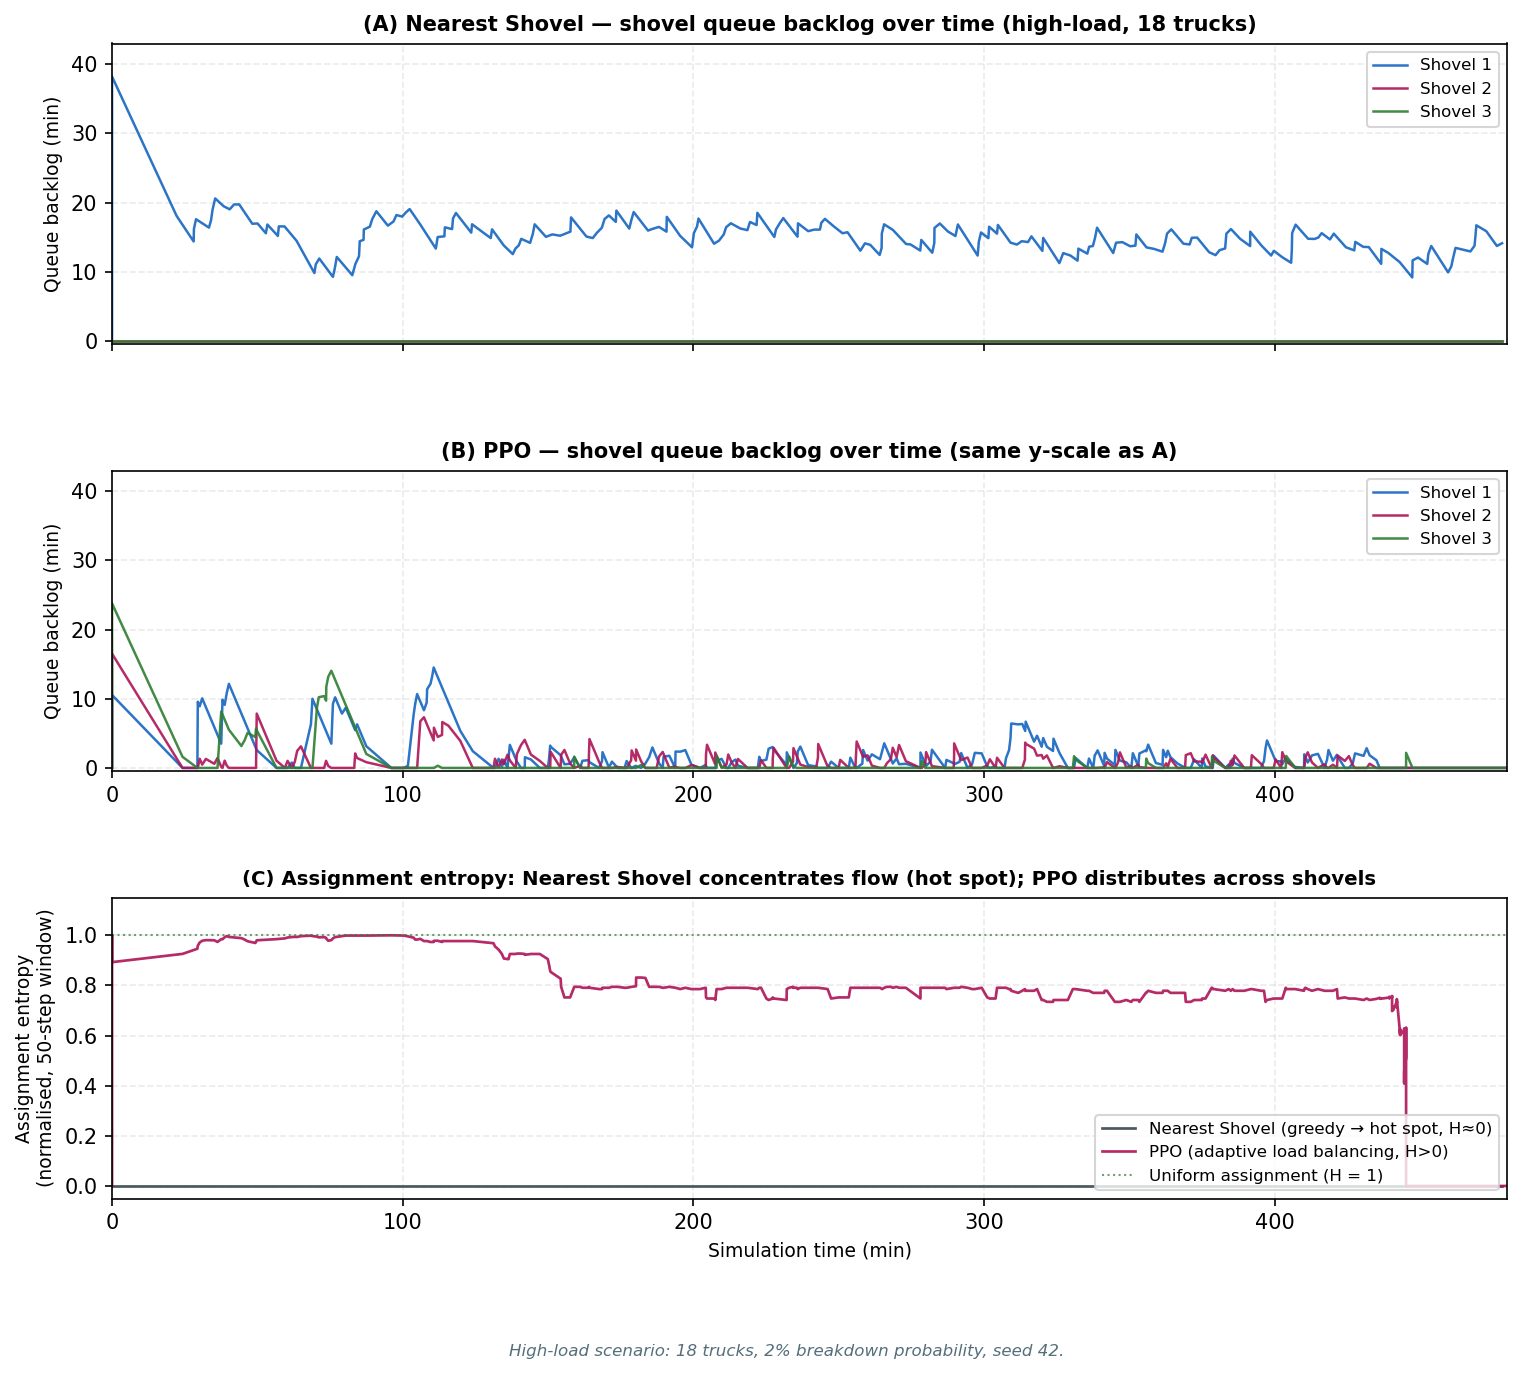
\includegraphics[width=0.96\textwidth]{figures/behavioral_analysis.png}
\caption{Analyse comportementale de Pelle la plus proche et de PPO en forte charge. Épisode unique avec 18 camions et la graine 42. Les panneaux (A) et (B) partagent la même échelle de l'axe $y$ ; le panneau (C) rapporte l'entropie d'affectation normalisée, où $H=1$ correspond à une affectation uniforme entre les pelles.}
\label{fig:behavioral}
\end{figure}

\subsection{Implications industrielles}

L'intégration du DRL dans les flottes minières doit être envisagée comme une couche de décision complémentaire plutôt que comme un remplacement complet des FMS existants.

\begin{itemize}
  \item \textbf{Mode recommandation :} dans un premier temps, les agents DRL devraient fonctionner en « mode recommandation », en fournissant des suggestions d'affectation optimisées à des dispatchers humains ou à des contrôleurs de transport autonomes. Cela permet une approche hybride dans laquelle l'IA gère la complexité tandis que les humains conservent la supervision.
  \item \textbf{Validation avant déploiement :} les écarts de performance importants observés d'un scénario à l'autre soulignent la nécessité d'une validation hors ligne rigoureuse à l'aide de jumeaux numériques avant toute mise en œuvre en conditions réelles.
  \item \textbf{Intervention humaine :} le maintien d'un contrôle humain reste essentiel, en particulier pendant la période de transition, afin de gérer les cas limites que la simulation n'a pas pu couvrir.
  \item \textbf{Application aux grandes flottes et aux jeux de données volumineux :} l'application de l'approche proposée à l'échelle industrielle (flottes de 50 à 200 camions, typiques des exploitations à ciel ouvert géantes) soulève des défis à la fois de calcul et de gestion des données. Sur le plan du calcul, l'architecture MLP plate utilisée ici passe mal à l'échelle avec la taille de la flotte : la dimension de l'état croît linéairement avec le nombre de camions, et le temps d'entraînement croît de façon surlinéaire avec le nombre de pas d'interaction nécessaires à la convergence pour des problèmes de plus grande taille. Un encodeur à réseau de neurones sur graphe (GNN) opérant sur le graphe du réseau routier répond au premier problème en partageant les paramètres entre les nœuds, tandis que la distribution du calcul par des architectures multi-agents répond au second. Sur le plan des données, les grandes flottes génèrent une télémétrie à haute fréquence (positions GPS, poids de la charge utile, profondeurs des files d'attente aux pelles à une résolution inférieure à la minute) dont le volume peut atteindre l'ordre du téraoctet sur une année d'exploitation sur un seul site minier. Le tampon de rejeu d'expériences de DQN est particulièrement bien adapté pour exploiter cette richesse de données : un préentraînement hors ligne sur des journaux historiques de dispatching suivi d'un ajustement fin en ligne en simulation pourrait réduire substantiellement la charge d'exploration et réduire l'écart entre simulation et réel (\textit{sim-to-real}). Cela est cohérent avec l'avantage de débit de DQN sur PPO en conditions de fortes pannes observé dans cette étude, et suggère que, s'il est confirmé à grande échelle, DQN pourrait être le candidat le plus déployable industriellement pour les grands sites miniers disposant de nombreuses données historiques, bien que cette extrapolation reste spéculative et doive être validée empiriquement.
\end{itemize}

\subsection{Durabilité}
\label{sec:sustainability}

Bien que cette étude se concentre principalement sur la productivité, ses implications en matière de durabilité sont significatives.
Le \cref{tab:efficiency} consolide le taux d'utilisation des équipements et la consommation spécifique de carburant dans les scénarios nominal (N), de forte charge (FC) et de fortes pannes (FP). Ces chiffres fournissent la base quantitative de la discussion ci-dessous ; les statistiques des tests $t$ de Welch par paires et les intervalles de confiance correspondants sont rapportés avec chaque comparaison.

\begin{table}[H]
\centering
\caption{Taux d'utilisation des équipements et consommation spécifique de carburant pour toutes les politiques et tous les scénarios, rapportés sous la forme moyenne $\pm$ écart-type sur 30 réplications.}
\label{tab:efficiency}
\footnotesize\setlength{\tabcolsep}{3pt}
\begin{tabular}{lcccccc}
\toprule
\multirow{2}{*}{\textbf{Politique}}
  & \multicolumn{3}{c}{\textbf{Utilisation (\%)}}
  & \multicolumn{3}{c}{\textbf{Carburant spécifique (L/t)}} \\
\cmidrule(lr){2-4}\cmidrule(lr){5-7}
  & \textbf{N} & \textbf{FC} & \textbf{FP}
  & \textbf{N}     & \textbf{FC}    & \textbf{FP} \\
\midrule
FIFO            & 96,2 & 93,7 & \textbf{91,7}  & $0{,}0534\pm0{,}0006$ & $0{,}0546\pm0{,}0004$ & $0{,}0555\pm0{,}0007$ \\
Aff. fixe       & \textbf{96,4} & \textbf{93,9} & 90,8  & $0{,}0431\pm0{,}0003$ & $\mathbf{0{,}0444\pm0{,}0004}$ & $0{,}0453\pm0{,}0006$ \\
Pelle la plus proche & 87,3 & 62,3 & 83,6  & $0{,}0430\pm0{,}0004$ & $0{,}0582\pm0{,}0006$ & $0{,}0445\pm0{,}0005$ \\
Plus court chemin & 86,8 & 61,3 & 83,1  & $0{,}0432\pm0{,}0004$ & $0{,}0588\pm0{,}0005$ & $0{,}0447\pm0{,}0006$ \\
Q-Learning      & 90,9 & 88,7 & 84,9  & $0{,}0482\pm0{,}0012$ & $0{,}0537\pm0{,}0010$ & $0{,}0534\pm0{,}0014$ \\
SARSA           & 89,0 & 78,6 & 86,6  & $0{,}0555\pm0{,}0009$ & $0{,}0612\pm0{,}0008$ & $0{,}0571\pm0{,}0014$ \\
DQN             & 91,7 & 90,5 & 85,8  & $\mathbf{0{,}0408\pm0{,}0006}$ & $0{,}0445\pm0{,}0004$ & $\mathbf{0{,}0419\pm0{,}0006}$ \\
PPO             & 94,5 & 79,5 & 86,0  & $0{,}0415\pm0{,}0006$ & $0{,}0475\pm0{,}0023$ & $0{,}0427\pm0{,}0008$ \\
\bottomrule
\end{tabular}
\end{table}

\begin{itemize}
  \item \textbf{Réduction du temps d'inactivité :} DQN maintient un temps d'attente moyen de 47,8~min en forte charge, comparable à FIFO (45,2~min) et à l'Affectation fixe (43,2~min) ; Pelle la plus proche (199,6~min) et Plus court chemin (204,3~min) s'effondrent en cas de saturation de la flotte. L'effondrement du taux d'utilisation de Pelle la plus proche et de Plus court chemin en forte charge (62,3\,\% et 61,3\,\%, contre 93,9\,\% pour l'Affectation fixe ; \cref{tab:efficiency}) quantifie le coût direct de la congestion en débit : les camions passent plus d'un tiers du poste inactifs en file d'attente au lieu de transporter.
  \item \textbf{Consommation spécifique et émissions potentielles :} DQN obtient la consommation spécifique de carburant la plus faible dans le scénario nominal ($0{,}0408$~L/t, IC à 95\,\%~$[0{,}0406\,;\,0{,}0409]$) et dans le scénario de fortes pannes ($0{,}0419$~L/t, IC à 95\,\%~$[0{,}0418\,;\,0{,}0421]$). Les tests $t$ de Welch corrigés par Holm confirment des avantages importants et statistiquement significatifs par rapport à l'Affectation fixe : en nominal $\Delta=-5{,}5\,\%$ ($p=3{,}00\times10^{-46}$, $d=3{,}50$, IC à 95\,\% de la différence~$[-0{,}0026\,;\,-0{,}0020]$~L/t) ; en fortes pannes $\Delta=-7{,}3\,\%$ ($p=2{,}92\times10^{-58}$, $d=3{,}95$, IC à 95\,\%~$[-0{,}0036\,;\,-0{,}0031]$~L/t). PPO surpasse également l'Affectation fixe en nominal ($\Delta=-3{,}9\,\%$, $p=3{,}60\times10^{-33}$, $d=2{,}41$) et en fortes pannes ($\Delta=-5{,}6\,\%$, $p=1{,}18\times10^{-36}$, $d=2{,}49$). En forte charge, DQN et l'Affectation fixe sont pratiquement à égalité ($0{,}0445$ contre $0{,}0444$~L/t ; IC à 95\,\%~$[0{,}0444\,;\,0{,}0446]$ contre $[0{,}0443\,;\,0{,}0445]$ ; $p=0{,}875$, n.s.), tandis que PPO consomme davantage ($0{,}0475$~L/t, $+7{,}0\,\%$, $p<0{,}001$, $d=2{,}15$), ce qui est cohérent avec son acheminement à forte variance en cas de saturation de la flotte. SARSA présente la pire efficacité en carburant dans tous les scénarios, reflétant ses temps d'attente plus longs et sa consommation plus élevée à l'arrêt. L'ampleur de la principale différence de carburant ($|\Delta|=0{,}0023$~L/t, DQN vs Affectation fixe en nominal) correspond à environ 53~L économisés par 1\,000 tonnes de minerai déplacées, une économie opérationnelle non négligeable au débit d'une mine. Les tailles d'effet exceptionnellement grandes ($d>3$) reflètent la faible variabilité intra-politique de la consommation de carburant (CV~$<5\,\%$) par rapport à la différence inter-politiques. Comme la combustion du diesel est la principale source d'émissions directes de CO$_2$, de NO$_x$ et de particules des flottes d'exploitation minière de surface, une politique qui réduit la consommation spécifique par tonne produirait en principe une réduction proportionnelle des émissions à l'échappement. Cependant, tous les chiffres rapportés ici sont issus de la simulation ; aucune mesure directe des émissions n'a été effectuée. Une validation de terrain sur un site minier réel est requise avant de pouvoir formuler toute affirmation définitive d'amélioration environnementale.
\end{itemize}

\subsection{Limites}
\label{sec:limitations}

Malgré la rigueur de cette étude, plusieurs limites doivent être reconnues :

\begin{itemize}
  \item \textbf{Écarts de simulation et absence de validation en mine réelle :} l'étude repose entièrement sur un environnement simulé et n'a pas été validée sur un site minier réel. Plusieurs facteurs ne peuvent pas être pleinement reproduits dans une simulation à événements discrets : conditions météorologiques et de visibilité imprévisibles, comportement variable des opérateurs, événements routiers non cartographiés et décisions de maintenance ponctuelles. Ces facteurs peuvent affecter substantiellement la transférabilité des gains de performance rapportés aux conditions opérationnelles.
  \item \textbf{Homogénéité de la flotte :} notre modèle suppose une flotte largement homogène. En pratique, les mines exploitent des camions d'âges et de capacités variés, ce qui ajoute une couche de complexité supplémentaire à la logique de dispatching.
  \item \textbf{Modèle de panne simplifié :} les pannes sont générées par un processus stochastique stationnaire et ne tiennent pas compte des dépendances liées à l'usure ni de la planification de la maintenance.
  \item \textbf{Espace d'actions discret :} l'agent est limité à un ensemble discret de pelles et de sites de déversement. Les travaux futurs devraient explorer des espaces d'actions continus ou hiérarchiques afin de mieux modéliser les intersections complexes et les exploitations multi-fosses.
  \item \textbf{Réseau routier relativement statique :} bien que les temps de trajet soient stochastiques et que les pistes se dégradent au fil du temps, la topologie du réseau lui-même reste fixe pendant un épisode.
  \item \textbf{Sélection des algorithmes :} cette étude s'est concentrée sur PPO, DQN et l'apprentissage par renforcement tabulaire. Plusieurs algorithmes compétitifs n'ont pas été inclus : Soft Actor-Critic (SAC) \cite{Haarnoja2018, SampsonNwachukwu2025}, Advantage Actor-Critic (A2C), Importance-Weighted Actor-Learner Architecture (IMPALA), et l'apprentissage par renforcement multi-agent (MARL) \cite{Zhao2025} pour la coordination décentralisée des camions. Des comparaisons avec ces méthodes représentent une piste importante pour les travaux futurs.
  \item \textbf{Budget d'entraînement des références tabulaires :} les agents tabulaires ont été entraînés pendant 30\,000 épisodes, un budget dans lequel ils n'atteignent pas de plateau de convergence (\cref{fig:convergence}). Leur performance rapportée est donc une borne inférieure, et l'écart entre agents tabulaires et profonds doit être lu comme un écart sous un budget pratique fixe plutôt que comme un écart entre optima convergés.
  \item \textbf{Budget de réplication :} bien que 30 réplications indépendantes par cellule (politique, scénario) offrent une puissance statistique suffisante pour les comparaisons rapportées ici, cela reste un plafond pratique. Les politiques à forte variance en cas de perturbation, notamment PPO en forte charge ($\pm$325~t/h, \cref{tab:productivity}), bénéficieraient d'un budget de réplication plus large pour resserrer davantage les intervalles de confiance.
  \item \textbf{Passage à l'échelle vers de grandes flottes et de grands jeux de données :} les expériences ont utilisé une flotte limitée (12 à 18 camions, 3 pelles) dont l'espace d'états peut être représenté de manière compacte. Le passage à des méga-mines exploitant 50 à 200 véhicules induit une explosion combinatoire qui rend les méthodes tabulaires (Q-Learning, SARSA) complètement intraitables et met en difficulté même les approches à approximation de fonction telles que DQN et PPO. Trois stratégies complémentaires sont identifiées pour les travaux futurs. (i)~\textit{Encodeurs à réseaux de neurones sur graphe (GNN)} : remplacer le MLP plat par un GNN opérant sur le graphe routier de la mine gère naturellement les tailles de flotte variables et généraliserait en principe à des topologies de mines jamais vues sans réentraînement à partir de zéro. (ii)~\textit{Apprentissage par renforcement multi-agent (MARL)} : décentraliser le dispatching de sorte que chaque camion agisse comme un agent indépendant avec des observations locales réduit l'espace d'actions conjoint de $\mathcal{O}(|\text{pelles}|^{N})$ à $\mathcal{O}(|\text{pelles}|)$ par camion, au prix d'une non-stationnarité pendant l'entraînement \cite{Zhao2025}. (iii)~\textit{Apprentissage par transfert et curriculum} : une politique entraînée sur une petite flotte de référence peut être ajustée finement sur une flotte plus grande en utilisant une fraction du budget d'entraînement total, à condition que l'encodage de l'état soit indépendant de la taille de la flotte. Du point de vue des données, les grandes flottes génèrent des journaux d'interaction proportionnellement plus riches (davantage de transitions par épisode), ce qui profite davantage aux méthodes à rejeu d'expériences telles que DQN qu'aux méthodes on-policy telles que PPO, en cohérence avec l'avantage de robustesse observé ici pour DQN en conditions de fortes pannes, dont l'attribution causale au mécanisme de rejeu reste à établir par ablation.
\end{itemize}

% ============================================================================
% Section 8: Conclusion
% ============================================================================
\section{Conclusion et travaux futurs}
\label{sec:conclusion}

Cette étude a abordé la question cruciale de savoir si les politiques d'apprentissage par renforcement profond peuvent améliorer la productivité et la résilience opérationnelle des systèmes camions--pelles par rapport aux heuristiques industrielles traditionnelles. En comparant huit politiques de dispatching distinctes dans trois régimes opérationnels stochastiques (nominal, forte charge et fortes pannes), nous avons fourni une évaluation complète de la logistique adaptative dans l'exploitation minière à ciel ouvert.

La méthodologie reposait sur un simulateur stochastique sur mesure d'une mine à ciel ouvert, fondé sur Gymnasium et intégrant des temps de trajet stochastiques et des modèles de panne d'équipements, ainsi que sur un protocole statistique fondé sur 30 réplications indépendantes, des graines aléatoires communes, l'ANOVA de Welch (scénario nominal) et Kruskal--Wallis (scénarios perturbés), des tests post-hoc de Dunn avec correction de Holm--Bonferroni, et des intervalles de confiance bootstrap. Les principaux résultats dressent un tableau nuancé. En conditions nominales, l'agent PPO a atteint la productivité la plus élevée (4\,176,67 t/h), soit une amélioration de 2,6\,\% par rapport à l'Affectation fixe, tandis que l'Affectation fixe elle-même a obtenu le temps d'attente moyen le plus faible (29,4 min), ce qui démontre que les politiques adaptatives et à base de règles sont compétitives sur des métriques différentes. En cas de sursaturation de la flotte, un \textit{effondrement par congestion} a été observé exclusivement pour les heuristiques fondées sur la distance (Pelle la plus proche : 199,6 min, Plus court chemin : 204,3 min), tandis que les heuristiques fondées sur les files d'attente (FIFO, Affectation fixe) et les agents DRL ont maintenu des temps d'attente inférieurs à 100 min. Enfin, DQN a obtenu le débit absolu le plus élevé dans le régime de fortes pannes (3\,949,17 t/h, $\Delta=4{,}49\,\%$), devançant PPO de 49,6~t/h ($d=0{,}636$, IC à 95\,\% $[21{,}4\,;\,77{,}8]$~t/h ; Welch $p=5{,}4\times10^{-4}$, bien que le test post-hoc principal de Dunn fondé sur les rangs donne $p=0{,}686$, bien au-dessus du seuil $\alpha=0{,}05$ et donc non significatif). Le tampon de rejeu d'expériences de DQN peut contribuer à cet avantage en permettant à l'agent de réutiliser les états de transition impliquant des événements de panne sur plusieurs mises à jour du gradient, un mécanisme indisponible pour l'agent PPO on-policy. Cela reste une hypothèse mécaniste cohérente avec les données plutôt qu'une affirmation causale confirmée. SARSA présente le meilleur ratio de robustesse relative ($\text{RR}_{\mathrm{FP}}=0{,}966$, $\Delta=3{,}38\,\%$), bien que cela reflète sa référence nominale plus basse plutôt qu'une véritable résilience adaptative. Parmi les politiques les plus performantes, PPO se dégrade le plus ($\Delta=6{,}63\,\%$), devant l'Affectation fixe ($\Delta=6{,}22\,\%$) et DQN ($\Delta=4{,}49\,\%$), tandis que Q-Learning ($\Delta=11{,}30\,\%$) illustre que le RL tabulaire ne se transfère pas bien à des dynamiques perturbées.

La principale contribution scientifique de cette recherche est de démontrer que la résilience opérationnelle constitue une dimension de performance à part entière, distincte de l'efficacité nominale. Nous avons montré que la stratégie de dispatching optimale dépend du régime : une stratégie qui excelle en conditions stables n'est pas nécessairement la plus robuste face aux perturbations. Ce résultat souligne la nécessité pour les systèmes de gestion de flotte de s'éloigner des règles d'optimisation locales et statiques pour aller vers des agents adaptatifs et globalement conscients, capables d'anticiper la propagation des retards dans le réseau de transport.

La principale limite de ce travail est l'absence de validation sur un site minier réel. Tous les résultats sont issus d'un simulateur stochastique sur mesure d'une mine à ciel ouvert ; l'écart entre simulation et réel persiste, en particulier en ce qui concerne le comportement imprévisible des opérateurs, la variabilité du terrain et les événements routiers non cartographiés. Un déploiement sur le terrain nécessitera une phase de calibration rigoureuse sur des données opérationnelles.

Par conséquent, les travaux futurs à court terme devraient se concentrer sur le développement de cadres d'apprentissage par renforcement hiérarchiques ou multi-agents dans lesquels chaque camion fonctionne comme un agent décentralisé doté d'une perception locale et d'une coordination globale. La prochaine étape de validation consistera à tester ces politiques sur un jumeau numérique calibré avec des données opérationnelles réelles d'un site minier actif. Une telle transition sera essentielle pour vérifier le passage à l'échelle des agents DRL à des centaines de véhicules et pour quantifier leur impact direct sur la consommation de carburant et les émissions de carbone dans un environnement minier physique. En définitive, cette recherche ouvre la voie à la prochaine génération de logistique minière autonome, résiliente et durable.

\newpage

% ============================================================================
% Sections finales
% ============================================================================
\section*{Disponibilité des données}

Les jeux de données synthétiques générés au cours de la présente étude, y compris les journaux de simulation et les indicateurs de performance pour les différents scénarios opérationnels, sont disponibles auprès de l'auteur correspondant sur demande raisonnable.

\section*{Disponibilité du code}

Le code source du simulateur stochastique de mine, les scripts d'entraînement et d'évaluation, les fichiers YAML d'hyperparamètres du répertoire \texttt{configs/}, et la liste exacte des graines utilisées pour les 30 réplications (graines 42--71) sont accessibles publiquement sur GitHub à l'adresse \url{https://github.com/Juan-Lucas/memoire-master-rl-logistique}.

\section*{Contributions des auteurs}

\textbf{Jean-Luc MUPASA KALUNGA :} conceptualisation, méthodologie, logiciel, validation, analyse formelle, investigation, rédaction (première version), visualisation.

\textbf{Dr Olfa FERCHICHI :} supervision, conceptualisation, méthodologie, rédaction (relecture et édition), administration du projet.

\section*{Conflit d'intérêts}

Les auteurs déclarent n'avoir aucun intérêt financier concurrent connu ni aucune relation personnelle susceptible d'avoir influencé les travaux rapportés dans cet article.

% Bibliographie
% \nocite{*}  % removed: all references are cited explicitly in the text
\bibliographystyle{plain}
\bibliography{RL_references}

% ============================================================================
% LISTE DES CLES DE CITATION UTILISEES (a verifier contre RL_references.bib)
% ---------------------------------------------------------
% Afrapoli2017            -> Afrapoli & Askari-Nasab, 2017 (FMS review)
% AlexandraNewman2010     -> Newman et al., 2010 (OR in mine planning)
% MohanMunirathinam1994   -> Munirathinam & Yingling, 1994
% Alarie2002              -> Alarie & Gamache, 2002
% Subtil2011              -> Subtil et al., 2011
% MehrnazMohtasham2023    -> Mohtasham & Mirzaei-Nasirabad, 2023
% NecmettinCetin2004      -> Cetin, 2004 (PhD thesis)
% MarceloFioroni2008      -> Fioroni et al., 2008
% Zeng2022                -> Zeng et al., 2022
% MiladAbolghasemian2020  -> Abolghasemian et al., 2020
% Soumis1989              -> Soumis et al., 1989
% Ahangaran2012           -> Ahangaran et al., 2012
% ChungTa2013             -> Ta et al., 2013
% AmandaSmith2020         -> Smith et al., 2020
% ZhongxinWang2022        -> Wang et al., 2022
% Souza2010               -> Souza et al., 2010
% GuangweiLiu2019         -> Liu & Chai, 2019
% BurakOzdemir2019        -> Ozdemir & Kumral, 2019
% ShivPrakashUpadhyay2017 -> Upadhyay & Askari-Nasab, 2017
% RichardSutton2018       -> Sutton & Barto, 2018
% MoezKrichen2022         -> Krichen, 2022
% MohammadrezaNazari2018  -> Nazari et al., 2018
% CongZhang2020           -> Zhang et al., 2020
% Hazrathosseini2024      -> Hazrathosseini & Afrapoli, 2024
% deCarvalho2023          -> de Carvalho & Dimitrakopoulos, 2023
% Banerjee2025            -> Banerjee et al., 2025 (Mining-Gym)
% Zhao2025                -> Zhao et al., 2025 (hierarchical MARL)
% Pei2025                 -> Pei et al., 2025
% FranciscoRosales2025    -> Rosales & Diaz, 2025
% JohnSchulman2017        -> Schulman et al., 2017 (PPO)
% MarkTowers2025          -> Towers et al., 2025 (Gymnasium)
% AntoninRaffin2021       -> Raffin et al., 2021 (Stable-Baselines3)
% SampsonNwachukwu2025    -> Nwachukwu et al., 2025 (SAC vs DDPG)
% KingaSzatmari2025        -> Szatmari et al., 2025 (cite en 2.3 et dans le tableau)
% ============================================================================

\end{document}
